\documentclass[a4paper,11pt,titlepage]{scrbook}
\usepackage[utf8]{inputenc}
\usepackage[spanish]{babel}
\usepackage{wrapfig}
\usepackage{float}
\usepackage{titlesec}

\setcounter{secnumdepth}{4}


\titleformat{\paragraph}
{\normalfont\normalsize\bfseries}{\theparagraph}{1em}{}
\titlespacing*{\paragraph}
{0pt}{3.25ex plus 1ex minus .2ex}{1.5ex plus .2ex}


%\usepackage{titlesec}
%\usepackage{palatino} %usar fot palatino en vez de times roman

%\decimalpoint %revisar
%\usepackage{dcolumn} %revisat
%\newcolumntype{.}{D{.}{\esperiod}{-1}}
%\makeatletter
%\addto\shorthandsspanish{\let\esperiod\es@period@code}
%\makeatother


%\usepackage[chapter]{algorithm}
%\RequirePackage{verbatim}
%\RequirePackage[Glenn]{fncychap}
\usepackage{fancyhdr}
\usepackage{graphicx}
\usepackage{afterpage}
\usepackage{longtable}
\usepackage{xcolor}
\definecolor{portada}{RGB}{239,206,53}
\definecolor{base}{RGB}{35,31,32}
\usepackage{pdfpages}
\usepackage[acronym]{glossaries}
\usepackage{acronym}
\usepackage{breakcites}
\usepackage{verbatim} 

\renewcommand{\glossaryname}{Glosario}
\renewcommand{\acronymname}{Acrónimos}

%Instrucciones para poder escribir código y mostrarlo de manera elegante:
\definecolor{gray97}{gray}{.97}
\definecolor{gray75}{gray}{.75}
\definecolor{gray45}{gray}{.45}
\definecolor{gray30}{gray}{.94}

\usepackage{listings}
\lstset{ frame=Ltb,
framerule=0pt,
aboveskip=0.5cm,
framextopmargin=3pt,
framexbottommargin=3pt,
framexleftmargin=0.4cm,
framesep=0pt,
rulesep=.4pt,
backgroundcolor=\color{gray97},
rulesepcolor=\color{black},
%
stringstyle=\ttfamily,
showstringspaces = false,
basicstyle=\small\ttfamily,
commentstyle=\color{gray45},
keywordstyle=\bfseries,
%
numbers=left,
numbersep=15pt,
numberstyle=\tiny,
numberfirstline = false,
breaklines=true,
literate={á}{{\'a}}1 {Á}{{\'A}}1 {é}{{\'e}}1 {É}{{\'e}}1 {í}{{\'i}}1  {Í}{{\'I}}1  {ó}{{\'o}}1  {Ó}{{\'O}}1  {ú}{{\'u}}1  {Ú}{{\'U}}1  {Ñ}{{\~N}}1 {ñ}{{\~n}}1 ,
}



% minimizar fragmentado de listados
\lstnewenvironment{listing}[1][]
   {\lstset{#1}\pagebreak[0]}{\pagebreak[0]}

\lstdefinestyle{Consola}
   {basicstyle=\scriptsize\bf\ttfamily,
    backgroundcolor=\color{gray30},
    frame=single,
    numbers=none
   }
\lstdefinestyle{C}
	{basicstyle=\scriptsize,
	frame=single,
	language=C,
	numbers=left
	}
\lstdefinestyle{CodigoC++}
        {basicstyle=\small,
	frame=single,
	backgroundcolor=\color{gray30},
	language=C++,
	numbers=left
 	}
\lstdefinestyle{PHP}
	{basicstyle=\scriptsize,
%        {basicstyle=\small,
	frame=single,
	language=PHP,
	numbers=left
	}
	



% ********************************************************************
% Información sobre el TFG. Comentar lo que NO se desee añadir y sustituir con la información correcta.
% ********************************************************************
\newcommand{\myTitle}{Creación de un videojuego de realidad virtual utilizando Unreal Engine 4}
%\newcommand{\mySubtitle}{Subtítulo del proyecto}
\newcommand{\myDegree}{Grado en Ingeniería Multimedia}
\newcommand{\myName}{José Luis Muñoz Periñán}
\newcommand{\myProf}{Francisco José Mora Lizán}
\newcommand{\myOtherProf}{Juan Antonio Puchol García}
\newcommand{\myFaculty}{Escuela Politécnica Superior de la Universidad de Alicante}
\newcommand{\myFacultyShort}{EPS UA}
\newcommand{\depTutorOne}{Dpto. de Ciencia de la Computación e Inteligencia Artificial}
\newcommand{\depTutorTwo}{Dpto. de Ciencia de la Computación e Inteligencia Artificial}

\newcommand{\nombreJuego}{"Nombre provisional"}

\newcommand{\myUni}{\protect{Universidad de Alicante}}
\newcommand{\myLocation}{Alicante}
\newcommand{\myTime}{\today}
%\newcommand{\myVersion}{Version 0.1}

\newcommand{\logoGrado}{imagenes/logoim.jpg}
\newcommand{\logoFacultad}{imagenes/logoeps.jpg}
\newcommand{\logoUniversidad}{imagenes/logoua.jpg}

\usepackage{url}

% Definición de comandos que me son útiles:
%\renewcommand{\indexname}{Índice alfabético}
%\renewcommand{\glossaryname}{Glosario}

\pagestyle{fancy}
\fancyhf{}
\fancyhead[LO]{\leftmark}
\fancyhead[RE]{\rightmark}
\fancyhead[RO,LE]{\textbf{\thepage}}
\renewcommand{\chaptermark}[1]{\markboth{\textbf{#1}}{}}
\renewcommand{\sectionmark}[1]{\markright{\textbf{\thesection. #1}}}


\setlength{\headheight}{1.5\headheight}

\newcommand{\HRule}{\rule{\linewidth}{0.5mm}}
%Definimos los tipos teorema, ejemplo y definición podremos usar estos tipos
%simplemente poniendo \begin{teorema} \end{teorema} ...
\newtheorem{teorema}{Teorema}[chapter]
\newtheorem{ejemplo}{Ejemplo}[chapter]
\newtheorem{definicion}{Definición}[chapter]
 
\newcommand{\bigrule}{\titlerule[0.5mm]}


%Para conseguir que en las páginas en blanco no ponga cabeceras
\makeatletter
\def\clearpage{%
  \ifvmode
    \ifnum \@dbltopnum =\m@ne
      \ifdim \pagetotal <\topskip
        \hbox{}
      \fi
    \fi
  \fi
  \newpage
  \thispagestyle{empty}
  \write\m@ne{}
  \vbox{}
  \penalty -\@Mi
}
\makeatother

\usepackage[pdfborder={000}]{hyperref} %referencia
\hypersetup{
	    colorlinks,
	linkcolor={blue!40!black},
	citecolor={blue!50!black},
	urlcolor={blue!80!black},
pdfauthor = {\myName (email (en) ua (punto) es)},
pdftitle = {\myTitle},
pdfsubject = {},
pdfkeywords = {palabra_clave1, palabra_clave2, palabra_clave3, ...},
pdfcreator = {LaTeX con el paquete ....},
pdfproducer = {pdflatex}
}
%AQUI COMIENZA LA LISTA DE FICHEROS A INCLUIR


\begin{document}
\renewcommand{\listtablename}{Índice de tablas} %para sustituir la palabra cuadro por tabla
\renewcommand{\tablename}{Tabla}
\renewcommand{\lstlistingname}{Listado}
\renewcommand{\lstlistlistingname}{Índice de \lstlistingname s}

\frontmatter
\begin{titlepage}

\newlength{\centeroffset}
\setlength{\centeroffset}{-0.5\oddsidemargin}
\addtolength{\centeroffset}{0.5\evensidemargin}
\thispagestyle{empty}
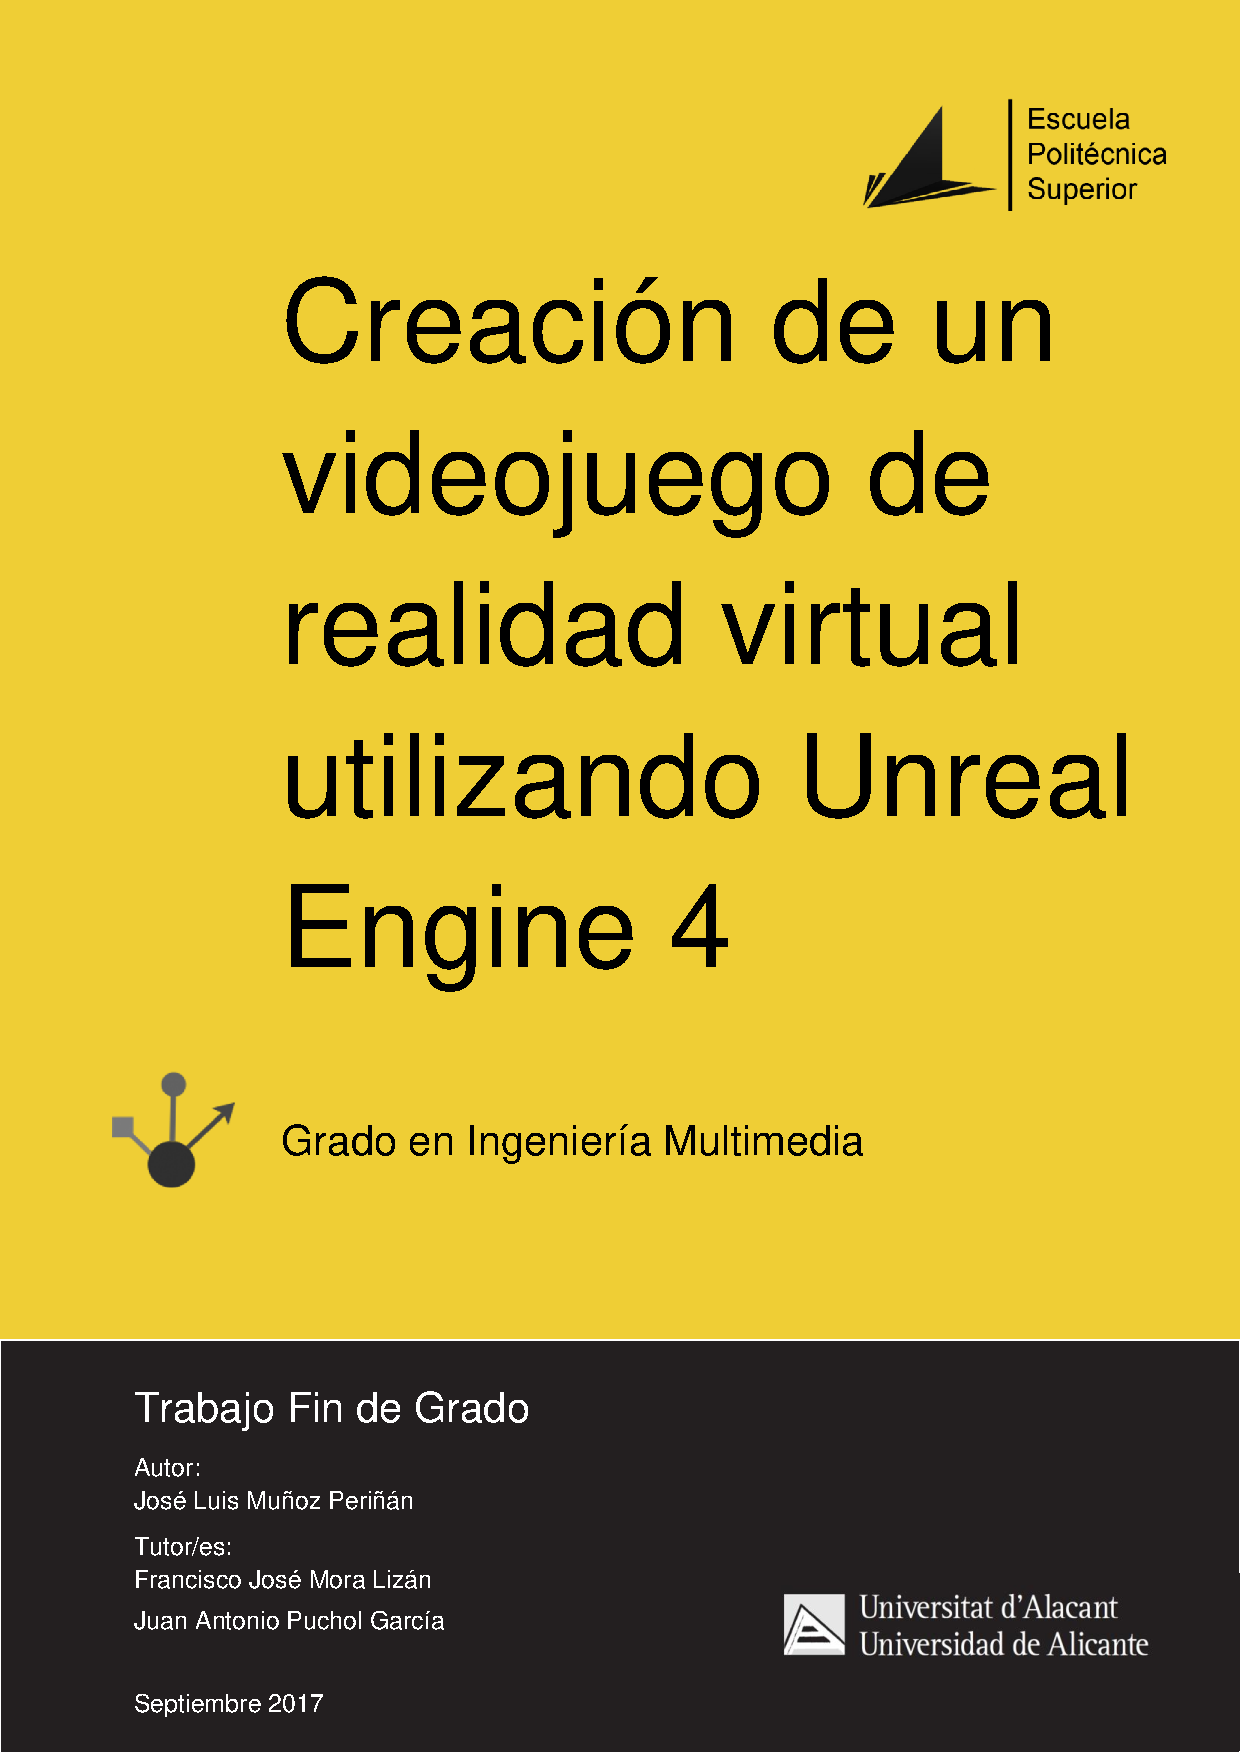
\includepdf[pages={1},pagecommand={},fitpaper=true,trim=0 0 0 0, 
offset=0 0,turn=true,noautoscale=true]{portada/portada.pdf}

\end{titlepage}
\pagecolor{white} %la portada en color
\begin{titlepage}
 
 
\setlength{\centeroffset}{-0.5\oddsidemargin}
\addtolength{\centeroffset}{0.5\evensidemargin}
\thispagestyle{empty}

\noindent\hspace*{\centeroffset}\begin{minipage}{\textwidth}

\centering


% Title

%{\Huge\bfseries Título del proyecto\\ }
{\Huge\bfseries \myTitle}

\noindent\rule[-1ex]{\textwidth}{3pt}\\[3.5ex]
%{\large\bfseries \mySubtitle\\[4cm]}
\end{minipage}

\vspace{2.5cm}
\noindent\hspace*{\centeroffset}\begin{minipage}{\textwidth}
\centering

\textbf{Autor}\\ {\myName}\\[2.5ex]
\textbf{Directores}\\
{\normalsize \myProf\\
\small\textit \depTutorOne\\
\normalsize \myOtherProf\\
\small\textit \depTutorTwo\\[2cm]}

\includegraphics[scale=0.25]{\logoGrado}


\textsc{\myDegree}\\

\centering
\begin{minipage}[l]{7cm}
\includegraphics[width=5cm]{\logoFacultad}
\end{minipage}
\begin{minipage}[r]{7cm}
\includegraphics[width=5cm]{\logoUniversidad}
\end{minipage}


%\textsc{\myFaculty}\\

%\large\bfseries \textsc{\myUni}\\
ALICANTE, \myTime

\end{minipage}
%\addtolength{\textwidth}{\centeroffset}
\vspace{\stretch{2}}

\end{titlepage}


 %la portada en b/n
\chapter*{Preámbulo}
\thispagestyle{empty}
Poner aquí un texto breve que debe incluir entre otras:
\begin{quote}
``las razones que han llevado a la realización del estudio, el tema, la finalidad y el alcance y también los agradecimientos por las ayudas, por ejemplo apoyo económico (becas y subvenciones) y las consultas y discusiones con los tutores y colegas de trabajo. \cite{UNE50136:97}''
\end{quote}

\cleardoublepage %salta a nueva página impar
% Aquí va la dedicatoria si la hubiese. Si no, comentar la(s) linea(s) siguientes
\chapter*{}
\setlength{\leftmargin}{0.5\textwidth}
\setlength{\parsep}{0cm}
\addtolength{\topsep}{0.5cm}
\begin{flushright}
\small\em{
A mi esposa Marganit, y a mis hijos Ella Rose y Daniel Adams,\\
sin los cuales habría podido acabar este libro dos años antes \footnote{Dedicatoria de Joseph J. Roman en ``An Introduction to Algebraic Topology''}
}
\end{flushright}


\cleardoublepage %salta a nueva página impar
% Aquí va la cita célebre si la hubiese. Si no, comentar la(s) linea(s) siguientes
\chapter*{}
\setlength{\leftmargin}{0.5\textwidth}
\setlength{\parsep}{0cm}
\addtolength{\topsep}{0.5cm}
\begin{flushright}
\small\em{
Si consigo ver más lejos\\
es porque he conseguido auparme\\ 
a hombros de gigantes
}
\end{flushright}
\begin{flushright}
\small{
Isaac Newton.
}
\end{flushright}
\cleardoublepage %salta a nueva página impar
 %editar este texto (capitulos/preliminares.tex) para cambiar preámbulo, agradecimientos y dedicatorias
\tableofcontents
\listoffigures
%\listoftables
%\lstlistoflistings

\mainmatter %entre frontmatter y mainmatter, la numeración es en romanos.

%a continuación se propone un esquema de trabajo que puede ser alterado justificadamente.
\acresetall{}  % resetea los acrónimos por si han sido usados en el índice o en los preliminares.
\chapter{Introducción}

Hoy en día la industria del videojuego es uno de los mercados más potentes de nuestra economía. Con el paso de los años este sector se ha ido extendiendo y normalizando hasta llegar al punto en el que se ha convertido en algo que aparece con total normalidad en nuestra vida cotidiana.

Hay todo tipo de juegos, desde sencillos juegos de móviles a grandes producciones que no tienen nada que enviar a las grandes películas con presupuestos millonarios de Hollywood, no es de extrañar que mucha gente considere el videojuego como \textit{el décimo arte.}

\section{Estructura de un \ac{TFG}}

En caso de que el \ac{TFG}/\acs{TFM} tenga como finalidad la elaboración de un proyecto o un 
informe científico o técnico, deberá ajustarse a lo dispuesto en las normas UNE 
157001:2002 y UNE 50135:1996 respectivamente.

Si el \ac{TFG}/\ac{TFM} tiene por finalidad la elaboración de un trabajo monográfico, el 
documento presentado deberá constar de las siguientes partes, teniendo como base la 
norma UNE 50136:1997.

\begin{description}
\item[Preámbulo:] se describirán brevemente la motivación que ha originado la realización del \ac{TFG}/\acs{TFM}, así como de una breve descripción de los objetivos generales que se quieren alcanzar con el trabajo presentado.
\item[Agradecimientos:] se podrá añadir las hojas necesarias para realizar los agradecimientos, a veces obligatorios, a las entidades y organismos colaboradores.
\item[Dedicatoria:] se podrá añadir una única hoja con dedicatorias, su alineación será derecha y centradas de forma distribuida en la página.
\item[Citas:] (frases célebres) se podrá añadir una única hoja con citas, su alineación será derecha y centradas de forma distribuida en la página.
\item[Índices:] cada índice debe comenzar en una nueva página, se incluirán los índices que se estimen necesarios (conforme UNE 50111:1989), en este orden:
\begin{description}
\item[Índice de contenidos:] (obligatorio siempre) se incluirá un índice de las secciones de las que se componga el documento, la numeración de las 
divisiones y subdivisiones utilizarán cifras arábigas (según UNE 50132:1994) y harán mención a la página del documento donde se ubiquen.
\item[Índice de figuras:] si el documento incluye figuras se podrá incluir también un índice con su relación, indicando la página donde se ubiquen.
\item[Índice de tablas:] en caso de existir en el texto, ídem que el anterior.
\item[Índice de abreviaturas, siglas, símbolos, etc.:] en caso de ser necesarios se podrá incluir cada uno de ellos.
\end{description}
\item[Cuerpo del documento:] en el contenido del documento se da flexibilidad para su organización y se puede estructurar en las secciones que se considere. En todo caso obligatoriamente se deberá, al menos, incluir los siguientes contenidos:
\begin{description}
\item[Introducción:] donde se hará énfasis a la importancia de la temática, su vigencia y actualidad; se planteará el problema a investigar, así como el propósito o finalidad de la investigación.
\item[Marco teórico o Estado del arte:] se hará mención a los elementos conceptuales que sirven de base para la investigación, estudios previos relacionados con el problema planteado, etc.
\item[Objetivos:] se establecerá el objetivo general y los específicos.
\item[Metodología:] se indicará el tipo o tipos de investigación, las técnicas y los procedimientos que serán utilizados para llevarla a cabo; se identificará la población y el tamaño de la muestra así como las técnicas e instrumentos de recolección de datos.
\item[Resultados:] incluirá los resultados de la investigación o trabajo, así como el análisis y la discusión de los mismos.
\end{description}
\item[Conclusiones:] obligatoriamente se incluirá una sección de conclusiones donde se realizará un resumen de los objetivos conseguidos así como de los resultados obtenidos si proceden.
\item[Bibliografía y referencias:] se incluirá también la relación de obras y materiales consultados y empleados en la elaboración de la memoria del \ac{TFG}/\ac{TFM}. La bibliografía y las referencias serán indexadas en orden alfabético (sistema nombre y fecha) o se numerará correlativamente según aparezca (sistema numérico). Se empleará la familia 1 como tipo de letra. Podrá utilizarse cualquier sistema bibliográfico normalizado predominante en la rama de conocimiento, estableciéndose como prioritarios el sistema ISO 690, sistema \ac{APA}  o Harvard (no necesariamente en ese orden de preferencia). En esta plantilla Latex se propone usar el estilo \ac{APA} indicándolo en la línea correspondiente como 
\begin{verbatim}
\bibliographystyle{apalike}
\end{verbatim}


\item[Anexos:] se podrá incluir los anexos que se consideren oportunos.

\end{description}




\chapter{Marco Teórico o  Estado del arte}
\label{marcoteorico}

En este apartado hablaré del concepto de videojuego y lo que define a un juego del género de terror. Para ello buscaré ejemplos en la industria, desde pequeños juegos realizados por estudios independientes (\textit{indies}) hasta grandes producciones de videojuegos realizadas por las principales empresas del sector.

\section{¿Que es un videojuego?}

Basta con buscar un poco por Internet para encontrar la siguiente definición de videojuego:
\\

\textit{Un videojuego es un juego electrónico en el que una o más personas interactúan, por medio de un controlador, con un dispositivo que muestra imágenes de vídeo. Este dispositivo electrónico puede ser una computadora, una máquina arcade, una videoconsola o un dispositivo portátil.}\footnote{Definición encontrada en la página de la Wikipedia: \url{https://es.wikipedia.org/wiki/Videojuego}.}
\\

Cada medio o autor usa sus propias palabras para definir lo que es un videojuego, sin embargo esta podría ser considerada la definición básica del término.
\\

A pesar de que ya habían juegos antes que ellos, los primeros videojuegos que triunfaron entre el gran público fueron juegos como \textit{Computer Space} (1971) o \textit{Pong} (1972). Este último tuvo especial éxito, siendo considerado como el juego más importante de la primera generación de videojuegos.
\\

El \textit{Pong} es un juego muy simple: es un juego de deportes de dos dimensiones que consiste en mover verticalmente una paleta para golpear una pelota y enviarla al campo del contrario. Cada vez que un jugador falla en golpear la bola el contrincante anota un punto, gana el jugador con más puntos.
\\


\begin{figure}
	\begin{center}
		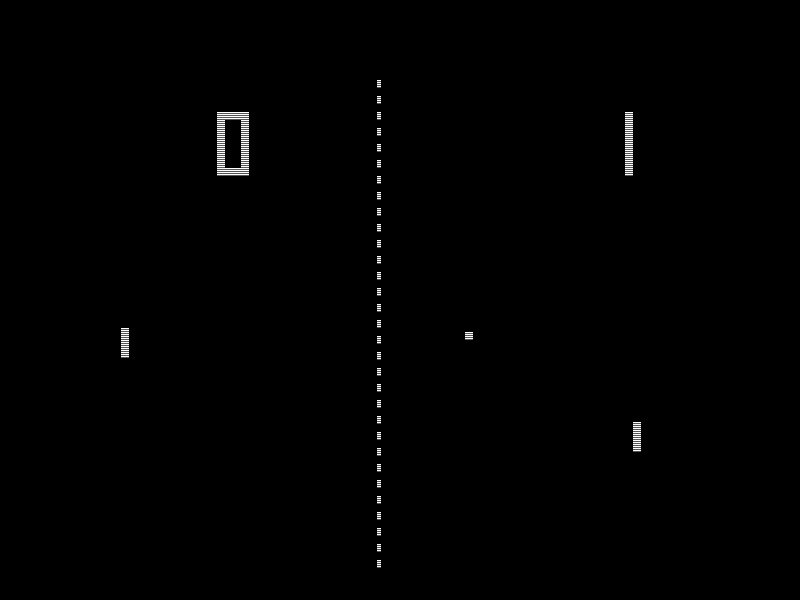
\includegraphics[scale=0.3]{imagenes/Pong.png}
		\caption{\textit{Pong}, el primer videojuego con un gran éxito comercial.}
		\label{spacewar}
	\end{center}
\end{figure}

El \textit{Pong} es un claro ejemplo de que con el paso de los años los videojuegos han evolucionado en todos los sentidos y se han hecho más accesibles entre el gran público. Al tener más éxito la industria ha concebido juegos cada vez más complejos.
\\

Hoy en día existen juegos de multitud de géneros como resultado de esa larga evolución, lejos queda ya esa época en la que el género Arcade eclipsaba todo el panorama de videojuegos, ahora existen un gran número de juegos capaces de contarte multitud de historias y con una amplia variedad de géneros y mecánicas.
\\


\section{Videojuego de terror}

El videojuego de terror ha evolucionado también mucho en los últimos años, los que podrían ser considerados los padres del género (como Resident Evil o Silent Hill) ya no tienen tanta relevancia en el espectro actual, aunque siguen siendo muy influyentes. 
\\

Para la realización de este videojuego se han observado y analizado un gran número de juegos de miedo, la mayoría son juegos recientes que aprovechan las últimas tendencias y cuyas mecánicas se pueden adaptar a la realidad virtual:

\begin{itemize}
	\item Outlast
	\item P.T.
	\item Alien: Isolation
	\item The Evil Within
	\item Resident Evil VII
\end{itemize}

\subsection{Outlast}

\begin{figure}
	\begin{center}
		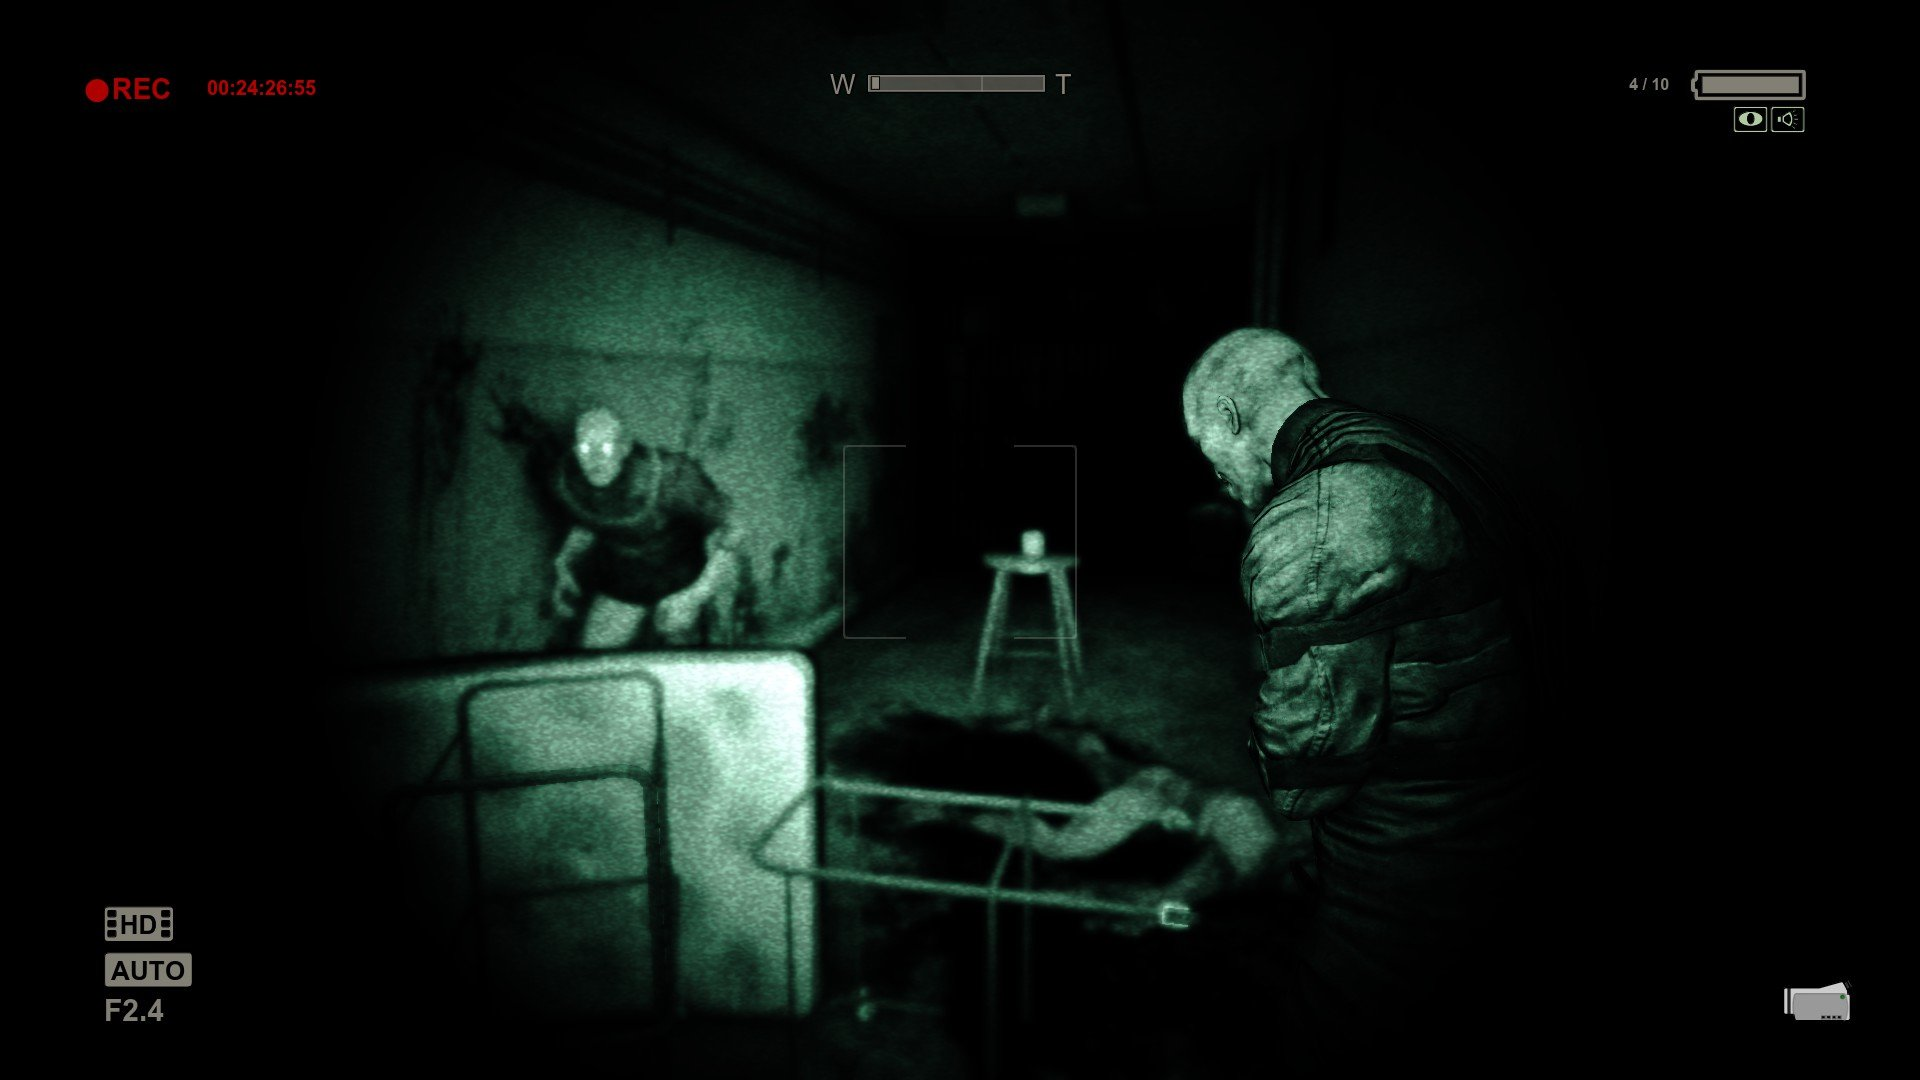
\includegraphics[scale=0.2]{imagenes/Outlast.jpg}
		\caption{Imagen \textit{in-game} de \textit{Outlast}.}
		\label{outlast}
	\end{center}
\end{figure}

Outlast es un videojuego de terror en primera persona desarrollado por el estudio canadiense \textit{Red Barrels Games} en 2013. En este juego eres un periodista encerrado en un psiquiátrico sobrenatural. 
\\

Este juego tiene varias mecánicas interesantes, en primer lugar, todo el juego gira en función a una cámara de vídeo que llevamos encima, ya que tiene visión nocturna y nos permite ver en los lugares más oscuros, por lo que es importante rastrear el escenario en busca de baterías para la cámara.
\\

Otro punto interesante de este juego es que no hay ninguna manera de atacar a los enemigos, por lo que siempre que te encuentras una amenaza tienes que huir. Esta mecánica, aunque puede llegar a ser frustrante, aumenta la sensación de infedensión, por lo que el miedo que se experimenta jugando es mucho mayor, ya que te sientes mucho más expuesto. Esta es una mecánica que me ha convencido y que se lleva practicando en algunos juegos desde hace un tiempo, por lo que he decidido implementarla en \textbf{\nombreJuego}.
\\

\subsection{P.T.}

\begin{figure}
	\begin{center}
		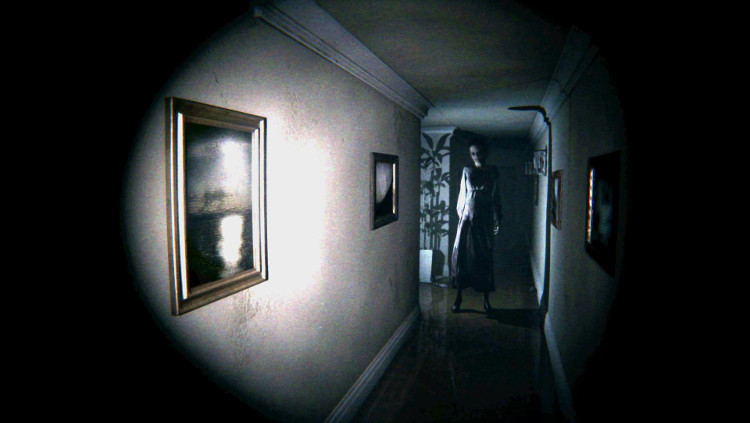
\includegraphics[scale=0.50]{imagenes/PT.jpg}
		\caption{Imagen \textit{in-game} de \textit{P.T.}}
		\label{PT}
	\end{center}
\end{figure}

Este juego me parece especialmente interesante, ya que no es un videojuego como tal, sino un \textit{teaser} de lo que iba a ser un nuevo \textit{Silent Hill} que nunca llego a ver la luz.
\\

Este juego fue desarrollado por \textbf{Hideo Kojima}, director de los famosos \textit{Metal Gear}, en colaboración con Guillermo Del Toro, director de películas como \textit{HellBoy} o \textit{Pacific Rim}. El juego estuvo disponible de manera gratuita durante un tiempo en 2014 y fue un éxito por parte del público y la crítica.
\\

Es un juego en tercera persona que transcurre en una pequeña casa donde ocurren fenómenos paranormales.Para superar el juego el jugador debe avanzar por las estancias de la casa superando algunos puzles. Este juego tampoco tiene una mecánica que implique usar la violencia, volviendo a esa sensación de indefensión que he mencionado anteriormente. Es un juego muy corto y que provoca un miedo principalmente atmosférico, causando una tensión constante en el jugador.
\\

Quiero destacar este juego porque me ha parecido especialmente interesante, sobre todo por la atmósfera y el arte, por lo que es uno de los principales referentes de \textbf{\nombreJuego}.
\\

\subsection{Alien: Isolation}

\begin{figure}
	\begin{center}
		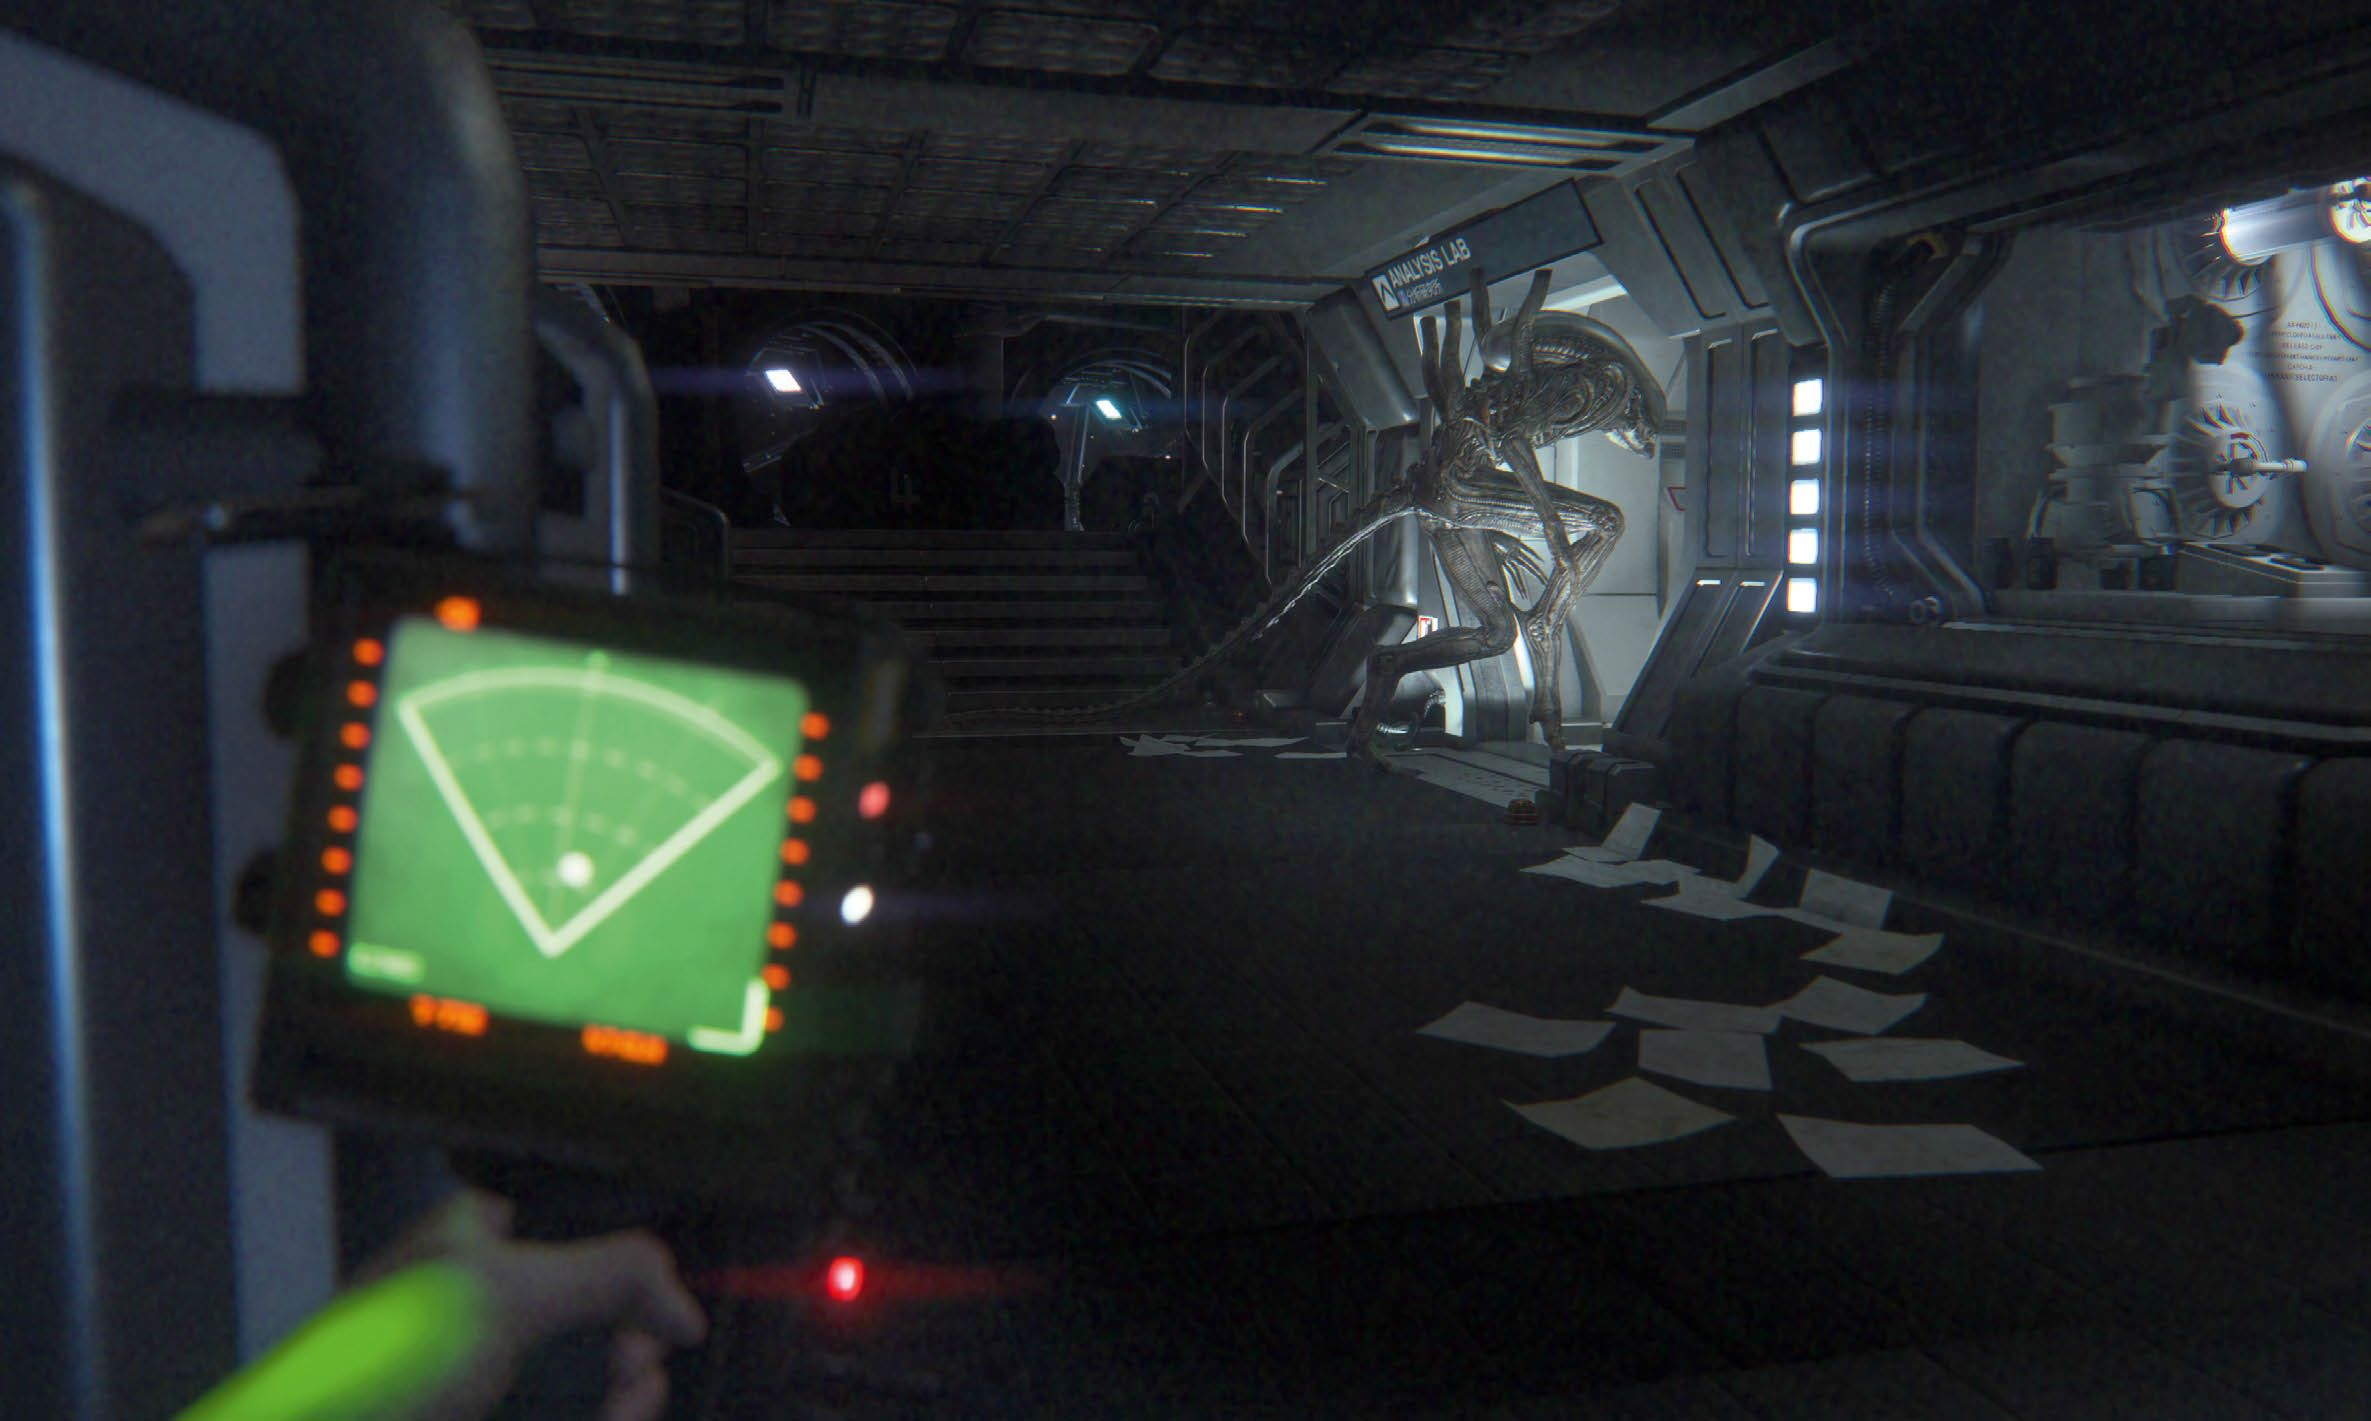
\includegraphics[scale=0.16]{imagenes/alien.jpg}
		\caption{Imagen \textit{in-game} de \textit{Alien: Isolation}.}
		\label{alien}
	\end{center}
\end{figure}

Este juego desarrollado por \textit{The Creative Assembly} en 2014 es un juego de terror y sigilo en primera persona basado en la franquicia de películas \textit{Alien}.
\\

Este juego transcurre en una nave destrozada en la que está libre el \textit{xenomorfo}, la principal mecánica del videojuego consiste en esconderse y escapar del alien. 
\\

Aunque en este juego si que dispones de herramientas para defenderte, a la hora de la verdad resultan inútiles contra el enemigo y tu mejor baza que tienes es escapar; otra vez más se repite ese sentimiento de desprotección, lo que aumenta considerablemente el miedo y la tensión al jugar.

\subsection{The Evil Within}

\begin{figure}
	\begin{center}
		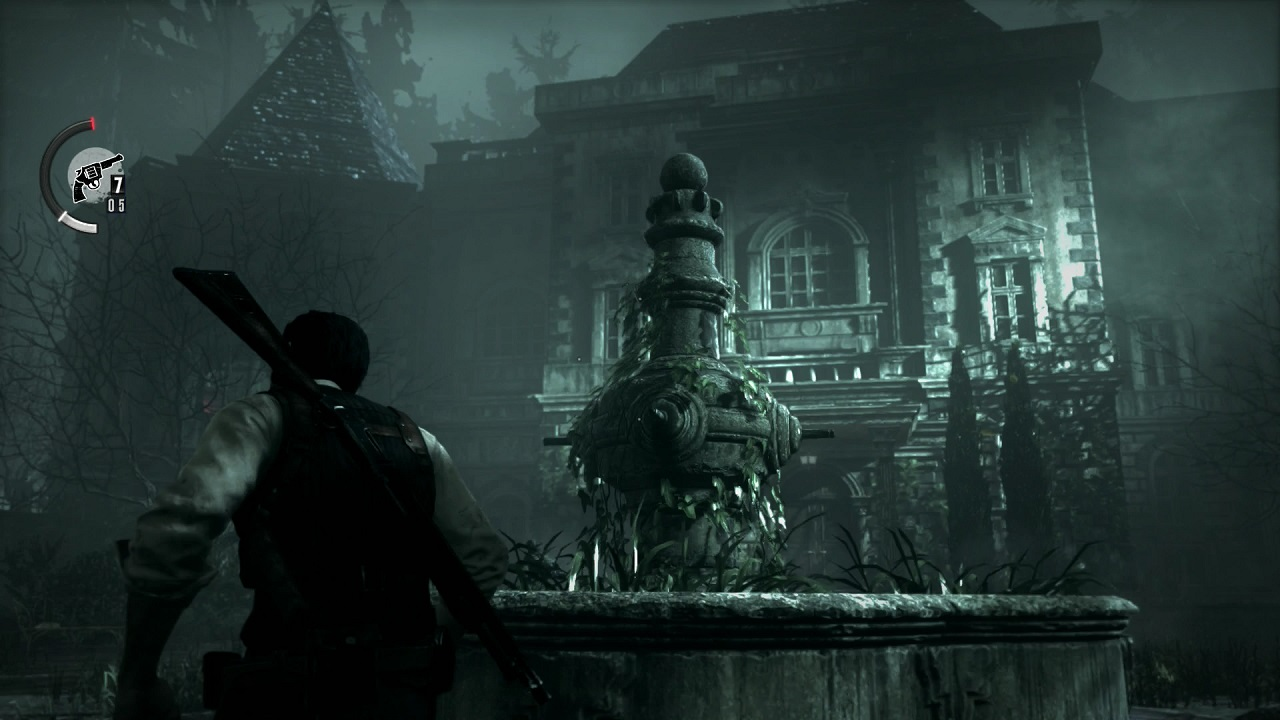
\includegraphics[scale=0.52]{imagenes/EvilWithin.jpg}
		\caption{Imagen \textit{in-game} de \textit{The Evil Within}.}
		\label{EvilWithin}
	\end{center}
\end{figure}

\textit{The Evil Within} es un juego bastante diferente a los anteriores, ya que incluye muchas mecánicas y partes de acción. No obstante es un juego destacable ya que ha tenido cierto éxito desde su salida en 2014.
\\

Este juego fue desarrollado por Shinji Mikami, creador de la saga \textit{Resident Evil}, unos de los padres del género. Es un juego de terror y acción en tercera persona, trata de un agente de policía que se tiene que enfrentar a ciertos fenómenos paranormales. En este juego te enfrentas directamente a muchos enemigos, usando armas de fuego o de cuerpo a cuerpo, además tienes que resolver un buen número de puzles para completar el juego.
\\

Este juego destaca entre otras cosas por lo grotesco de los enemigos y los escenarios, cuenta con un apartado artístico muy desagradable, proporcionando una sensación de incomodidad constante al jugador. Esto último resulta muy interesante, pero he decidido no incluir nada parecido en \nombreJuego, ya que las características de los juegos que he hablado anteriormente me han convencido más. No obstante, me ha parecido un juego con algunas propuestas interesantes e ideas que se pueden adaptar a \textbf{\nombreJuego}.

\subsection{Resident Evil VII}

\begin{figure}
	\begin{center}
		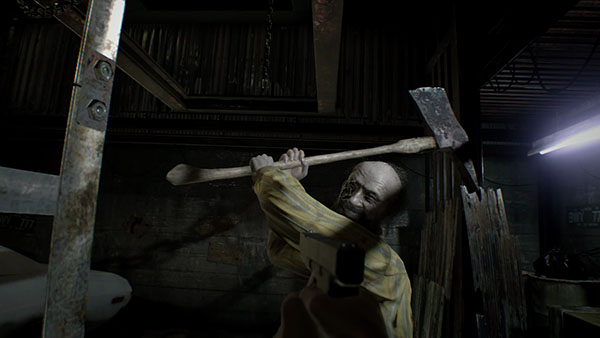
\includegraphics[scale=0.65]{imagenes/REVII.jpg}
		\caption{Imagen \textit{in-game} de \textit{Resident Evil VII}.}
		\label{ResidentEvil}
	\end{center}
\end{figure}

Para concluir este apartado, quiero mencionar el que es el principal referente para \textbf{\nombreJuego} junto a P.T. El Resident Evil VII es un juego que salió el pasado año y que supone la vuelta de la principal franquicia de juegos de terror.
\\

Este es un juego muy interesante, ya que toma las principales mecánicas de los juegos de terror en los últimos años y se adapta a ellas manteniendo la esencia de la franquicia.
\\

Es un juego en primera persona con mecánicas de acción con disparos que se desarrolla en una mansión. Para avanzar por la casa tienes que ir resolviendo ciertos puzles que desbloquean nuevas estancias y que hacen que avance la trama del juego. En este sentido el juego es muy semejante a P.T., ya que ambos juegos desarrollan la acción en un recinto cerrado donde la ambientación y la atmósfera de la casa ponen en una tensión constante al jugador.
\\
Quiero destacar además que este juego es totalmente compatible con dispositivos de realidad virtual, estando ya disponible para las gafas \textit{Playstation VR} y en un futuro para otros dispositivos.
\\








\begin{comment}
El contenido de este capítulo es una especie de muestrario de cosas que puedes hacer con \LaTeX.  Por ejemplo, incluir una cita bibliográfica   \cite{BOE_IM_UA} dentro del texto. En esta página de demostración también puedes encontrar información útil acerca de cómo escribir con  \LaTeX.\footnote{En http://metodos.fam.cie.uva.es/~latex/apuntes/apuntes.html hay unos buenos apuntes al respecto.}
\section{Listas}
Hacer una lista es simple en \LaTeX. Para ello has de crear un entorno (así se llama) itemize con
\begin{verbatim}
\begin{itemize}
...
\end{itemize}
\end{verbatim}
Y dentro de esa estructura, añadir cada elemento de la lista precedido de 
\begin{verbatim}
\item primer item de lista
\item segundo item de lista
...
\item ultimo item de lista
\end{verbatim}

Es importante que revises este texto tal como aparece en la plantilla y relaciones el aspecto que tiene el PDF final con cómo está escrito el documento \LaTeX.

Aquí va una lista:
\begin{itemize}
    \item Ingeniería Informática.
    \item Ingeniería Sonido e Imagen en Telecomunicación.
    \item Ingeniería Multimedia.
    \begin{itemize}
         \item Mención: Creación y ocio digital.
         \item Mención: Gestión de Contenidos.
    \end{itemize}
\end{itemize}


\section{Tablas}
Ahora veremos otra estructura más: las tablas.

\subsection{Inserción de tablas}

Aquí va una tabla\footnote{En http://www.tablesgenerator.com/ se puede encontrar un generador On-Line de tablas para \LaTeX} para que se vea cómo insertar una tabla simple dentro del documento.

\begin{table}[h]
\begin{center}
\begin{tabular}{lllll}
&columna A&columna B&columna C\\
\hline
fila 1&fila 1, columna A & fila 1, columna B & fila 1, columna C\\
fila 2&fila 2, columna A & fila 2, columna B & fila 2, columna C\\
fila 3&fila 3, columna A & fila 3, columna B & fila 3, columna C\\ \hline
\end{tabular}
\end{center}
\caption{Ejemplo de tabla.}
\label{tabladeejemplo}
\end{table}

\LaTeX usa un sistema de parámetros para ``decorar'' las tablas. Puedes consultar estos parámetros en la tabla \ref{tabla_parametros} de la página \pageref{tabla_parametros}. La tabla se ubicará donde, a juicio de \LaTeX, menos moleste por lo que puede no aparecer necesariamente donde se ha insertado en el texto original. 

\begin{table}
\begin{center}
\begin{tabular}{|c|p{0.8\textwidth}|}
\hline
Parámetro & \multicolumn{1}{c|}{Significado} \\ \hline
\texttt{h} & Situa el elemento flotante \emph{preferentemente}
(es decir, si es posible) en la situación exacta donde se incluye este \\
\texttt{t} & Situa el elemento en la parte de arriba de la página \\
\texttt{b} & Situa el elemento en la parte de abajo de la página \\
\texttt{p} & Situa el elemento en una página aparte dedicada sólo a
elementos flotantes; en el caso del formato \texttt{article},
ésta se situa al final del documento, mientras que para al book es
colocada al final de cada capítulo \\ \hline
\end{tabular}
\end{center}
\caption{Parámetros optativos de los entornos flotantes}
\label{tabla_parametros}
\end{table}



\section{Inserción de figuras}

Las figuras son un caso un poco especial ya que \LaTeX busca el mejor lugar para ponerlas, no siendo necesariamente el ligar donde está la referencia. Por ello es importante añadirle un ``caption'' y un ``label'' para poder hacer referencia a ellas en el párrafo correspondiente. Nosotros ponemos la referencia a la figura \ref{logo_im} que está en la página \pageref{logo_im}. justo aquí debajo, pero \LaTeX puede que la ubique en otro lugar.

\begin{figure}
\begin{center}

\includegraphics[scale=0.25]{imagenes/logoim.jpg}
\caption{Logo de Ingeniería  Multimedia.}
\label{logo_im}
\end{center}
\end{figure}

\begin{figure}
\begin{center}

\includegraphics[scale=0.25]{imagenes/logoeps.jpg}
\caption{Logo de la EPS.}
\label{logo_eps}
\end{center}
\end{figure}

\section{Inserción de código}
A veces tendrás que insertar algún pedazo de código fuente para explicar algo relacionado con él. No sustituyas explicaciones con enormes listados de código. Si pones algo de código en tu TFG que sea para demostrar algo o explicar alguna solución.

\LaTeX te ayuda a escribir código de manera que su presentación tenga las marcas y tabulaciones propias de este tipo de texto. Para ello, debes poner el código que escribas DENTRO de un entorno  que se llama ``listings''.  La plantilla ya tiene una serie de instrucciones para incluir el paquete ``listings'' y añadirle algunos modificadores por lo que no tienes que incluirlo tú. Simplemente, mete tu código en el entorno ``lstlisting'' y ya está. Puedes indicar el lenguaje en el que está escrito el código y así \LaTeX lo mostrará mejor. Veamos un ejemplo en la figura \ref{C_code}:

Si pones 
\begin{verbatim}
\begin{lstlisting}[style=C, caption={ejemplo código C},label=C_code]
#include <stdio.h>
int main(int argc, char* argv[]) {
  puts("Hola mundo!");
}
\end{lstlisting}
\end{verbatim}

El resultado será:
\begin{lstlisting}[style=C, caption={ejemplo código C},label=C_code]
#include <stdio.h>
int main(int argc, char* argv[]) {
  puts("Hola mundo!");
}
\end{lstlisting}

Por supuesto, puedes mejorar esta presentación utilizando mas modificadores. Esta información y mucha más puede ser encontrada en \cite{listing_packagge} y en \cite{heinz1listings}.

Otro ejemplo, ahora para mostrar código PHP, sería escribir en tu fichero \LaTeX lo siguiente:
\begin{verbatim}
 \begin{lstlisting}[style=PHP, caption={ejemplo código PHP},label=PHP_code]
 /* 
Ejemplo de código en PHP para escribir tu primer programa en este lenguaje
Copia este código en tu ordenador y ejecútalo
*/
<html>
  <head>
    <title>Prueba de PHP</title>
  </head>
  <body>
    <?php echo '<p>Hola Mundo</p>'; ?> //esto lo escribe TODO el mundo
  </body>
</html>
 \end{lstlisting}
\end{verbatim}
 
 y el resultado es: (ver listado \ref{PHP_code})
 
 \begin{lstlisting}[style=PHP, caption={ejemplo código PHP},label=PHP_code]
/* 
Ejemplo de código en PHP para escribir tu primer programa en este lenguaje. Copia este código en tu ordenador y ejecútalo
*/
 <html>
  <head>
    <title>Prueba de PHP</title>
  </head>
  <body>
    <?php echo '<p>Hola Mundo</p>'; ?> //esto lo escribe TODO el mundo
  </body>
</html>
 \end{lstlisting}
 
 Observa cómo \LaTeX ha puesto los comentarios en gris y ajustado el código para que se muestre más claro.
 
 Si quieres añadir código en otros lenguajes, cambia el comando que dice 
 
 \begin{center}
 ``style=nombredellenguaje''
 
  por 
 
 ``languaje=nombredelnuevolenguaje''.
 \end{center}
 
 \section{Acrónimos}
 Por último vamos a ver cómo se ponen los acrónimos.
 
 La norma dice que la primera vez que aparece un acrónimo debe ponerse su fórmula completa es decir, lo que significa, al lado del acrónimo. Después de ello, podemos usar ya sólo el acrónimo salvo cuando consideremos que debemos volver a usar la fórmula completa por alguna razón de legibilidad.
 
 ¿Cómo llevar la cuenta de cuándo es la primera vez que ponemos el acrónimo? si hacemos cambios en el doc es fácil que perdamos esa información así que lo mejor es que sea el propio \LaTeX  el que lleve esa cuenta. Para ello tenemos que hacer dos cosas:
 \begin{description}
 \item[Primero:] creamos la entrada del acrónimo en el fichero acronimos.tex. Revisad los comentarios de su cabecera para saber cómo crear esa entrada. Básicamente lo que hacemos allí es poner la ``fórmula corta'' y la ``fórmula larga'' del acrónimo es decir, el propio acrónimo y su significado
 \item[Segundo:] escribimos en el texto el acrónimo SIEMPRE diciendo que es un acrónimo y el tipo de fórmula que queremos usar. Por ejemplo, si siempre que queremos hacer referencia al IEEE escribimos \begin{verbatim}\ac{IEEE}\end{verbatim}  se consigue que la primera vez que aparezca el acrónimo ponga las fórmulas larga y la corta y en las siguientes ocasiones sólo aparecerá la corta.
 \end{description}
 
 Aquí va un ejemplo:
 
 Si escribimos:
 
 \begin{verbatim}
 El \ac{IEEE} es una institución muy importante en el mundo de la
 ingeniería.  El \ac{IEEE} lleva marcando normas y protocolos desde
 hace mucho tiempo.  Pero el \acf{IEEE} no está solo en esta tarea. 
 Además del \ac{IEEE} hay muchas otras instituciones para ello.
 \end{verbatim}
 
 Obtendremos: 
 
El \ac{IEEE} es una institución muy importante en el mundo de la ingeniería. El \ac{IEEE} lleva marcando normas y protocolos desde hace mucho tiempo. Pero el \acl{IEEE} no está solo en esta tarea. Además del \ac{IEEE} hay muchas otras instituciones para ello.

\end{comment}
 
\chapter{Objetivos}

El objetivo de este proyecto es la creación de un videojuego de terror para PC con la mayor calidad posible compatible con realidad virtual. Para esto se utilizará el motor comercial \textit{Unreal Engine 4}, programando todo lo necesario usando el sistema de \textit{Blueprint visual scripting}. Por tanto, otro objetivo en este \ac{TFG} es el aprendizaje de las diferentes funciones y características del motor \textit{Unreal Engine}.
\\

Además será necesario redactar un \ac{GDD} donde se realizará el diseño previo del videojuego, se analizarán grandes títulos del género para conseguir mayor calidad en el producto final y se crearán los recursos necesarios que serán incluidos en el videojuego, así como modificaciones de los recursos obtenidos de terceros con licencias que me permitan incluirlos en el juego.
\\


\section{Desglose de objetivos}

Estos son los objetivos del \ac{TFG} ordenados y puestos de manera más específica: 

\begin{enumerate}
	\item Realizar el \ac{GDD} del videojuego.
	\item Crear el videojuego base usando el sistema de \textit{blueprints} de \textit{Unreal}.
	\item Crear los modelos necesarios para el videojuego.
	\item Texturizar e incorporar los modelos en el juego.
	\item Importar los recursos de terceros necesarios y que lo permitan según sus licencias.
	\item Completar la lógica del videojuego usando \textit{blueprints}.
	\item Implementar los menús y el \textit{HUD}.
	\item Incorporar sonidos en el juego.
	\item Compatibilizar el juego con el dispositivo de realidad virtual de\textit{ Oculus Rift}.
\end{enumerate}


\begin{comment}


\begin{description}
\item[Índice de contenidos:] (obligatorio siempre) se incluirá un índice de las secciones de las que se componga el documento, la numeración de las 
divisiones y subdivisiones utilizarán cifras arábigas (según UNE 50132:1994) y harán mención a la página del documento donde se ubiquen.
\item[Índice de figuras:] si el documento incluye figuras se podrá incluir también un índice con su relación, indicando la página donde se ubiquen.
\item[Índice de tablas:] en caso de existir en el texto, ídem que el anterior.
\item[Índice de abreviaturas, siglas, símbolos, etc.:] en caso de ser necesarios se podrá incluir cada uno de ellos.
\end{description}
\item[Cuerpo del documento:] en el contenido del documento se da flexibilidad para su organización y se puede estructurar en las secciones que se considere. En todo caso obligatoriamente se deberá, al menos, incluir los siguientes contenidos:
\begin{description}
\item[Introducción:] donde se hará énfasis a la importancia de la temática, su vigencia y actualidad; se planteará el problema a investigar, así como el propósito o finalidad de la investigación.
\item[Marco teórico o Estado del arte:] se hará mención a los elementos conceptuales que sirven de base para la investigación, estudios previos relacionados con el problema planteado, etc.
\item[Objetivos:] se establecerá el objetivo general y los específicos.
\item[Metodología:] se indicará el tipo o tipos de investigación, las técnicas y los procedimientos que serán utilizados para llevarla a cabo; se identificará la población y el tamaño de la muestra así como las técnicas e instrumentos de recolección de datos.
\item[Resultados:] incluirá los resultados de la investigación o trabajo, así como el análisis y la discusión de los mismos.
\end{description}
\item[Conclusiones:] obligatoriamente se incluirá una sección de conclusiones donde se realizará un resumen de los objetivos conseguidos así como de los resultados obtenidos si proceden.
\item[Bibliografía y referencias:] se incluirá también la relación de obras y materiales consultados y empleados en la elaboración de la memoria del \ac{TFG}/\ac{TFM}. La bibliografía y las referencias serán indexadas en orden alfabético (sistema nombre y fecha) o se numerará correlativamente según aparezca (sistema numérico). Se empleará la familia 1 como tipo de letra. Podrá utilizarse cualquier sistema bibliográfico normalizado predominante en la rama de conocimiento, estableciéndose como prioritarios el sistema ISO 690, sistema \ac{APA}  o Harvard (no necesariamente en ese orden de preferencia). En esta plantilla Latex se propone usar el estilo \ac{APA} indicándolo en la línea correspondiente como 
\begin{verbatim}
\bibliographystyle{apalike}
\end{verbatim}


\item[Anexos:] se podrá incluir los anexos que se consideren oportunos.
\end{comment}






\chapter{Metodología}

A continuación hablaré de la gestión del proyecto y la metodología del desarrollo, así como del control de versiones y repositorio de este \ac{TFG}.

\section{Metodología del desarrollo}

Para el desarrollo del desarrollo de este proyecto he usado la metodología \textit{Kanban}, una metodología ágil basada en tableros y etiquetas. Para ello usaremos \textit{Trello}, una herramienta de gestión de proyectos que utiliza esta metodología de manera cómoda y práctica.

\subsection{¿Qué es Kanban?}

\textit{\textbf{Kanban}} es una metodología ágil creada hace muchos años en el seno de \textit{Toyota} y que ha sido usada durante décadas para mantener la línea de producción.
\\

Se basa en las siguientes ideas:

\begin{itemize}
	\item Permite tener una visualización del trabajo realizado.
	\begin{itemize}
		\item Divide todo el trabajo en ítems o tarjetas.
		\item Utiliza diferentes columna para poder visualizar en que parte del flujo de trabajo está cada ítem.
	\end{itemize}
	\item Mide y gestiona el flujo de trabajo.
	\item Permite identificar oportunidades de mejora.
\end{itemize}


Es una metodología muy útil y adecuada para este proyecto, ya que está pensada para equipos pequeños y que permite cambios imprevistos con mayor facilidad que otras metodologías.
\\

Un ejemplo de uso de esta metodología es el siguiente:

\begin{enumerate}
	\item Se crean tarjetas con tareas a realizar.
	\item Se mueven esas tarjetas a la columna \textit{Working} una vez que se empieza a trabajar con ellas.
	\item Cuando se termina con esa tarea se mueve la tarjeta a la columna \textit{Done}.
	\item Por último, se vuelve a escoger tareas en las que trabajar y se repite los pasos anteriores, así hasta la finalización del proyecto.
\end{enumerate}
	
\section{Gestión del proyecto}

\begin{figure}
	\begin{center}
		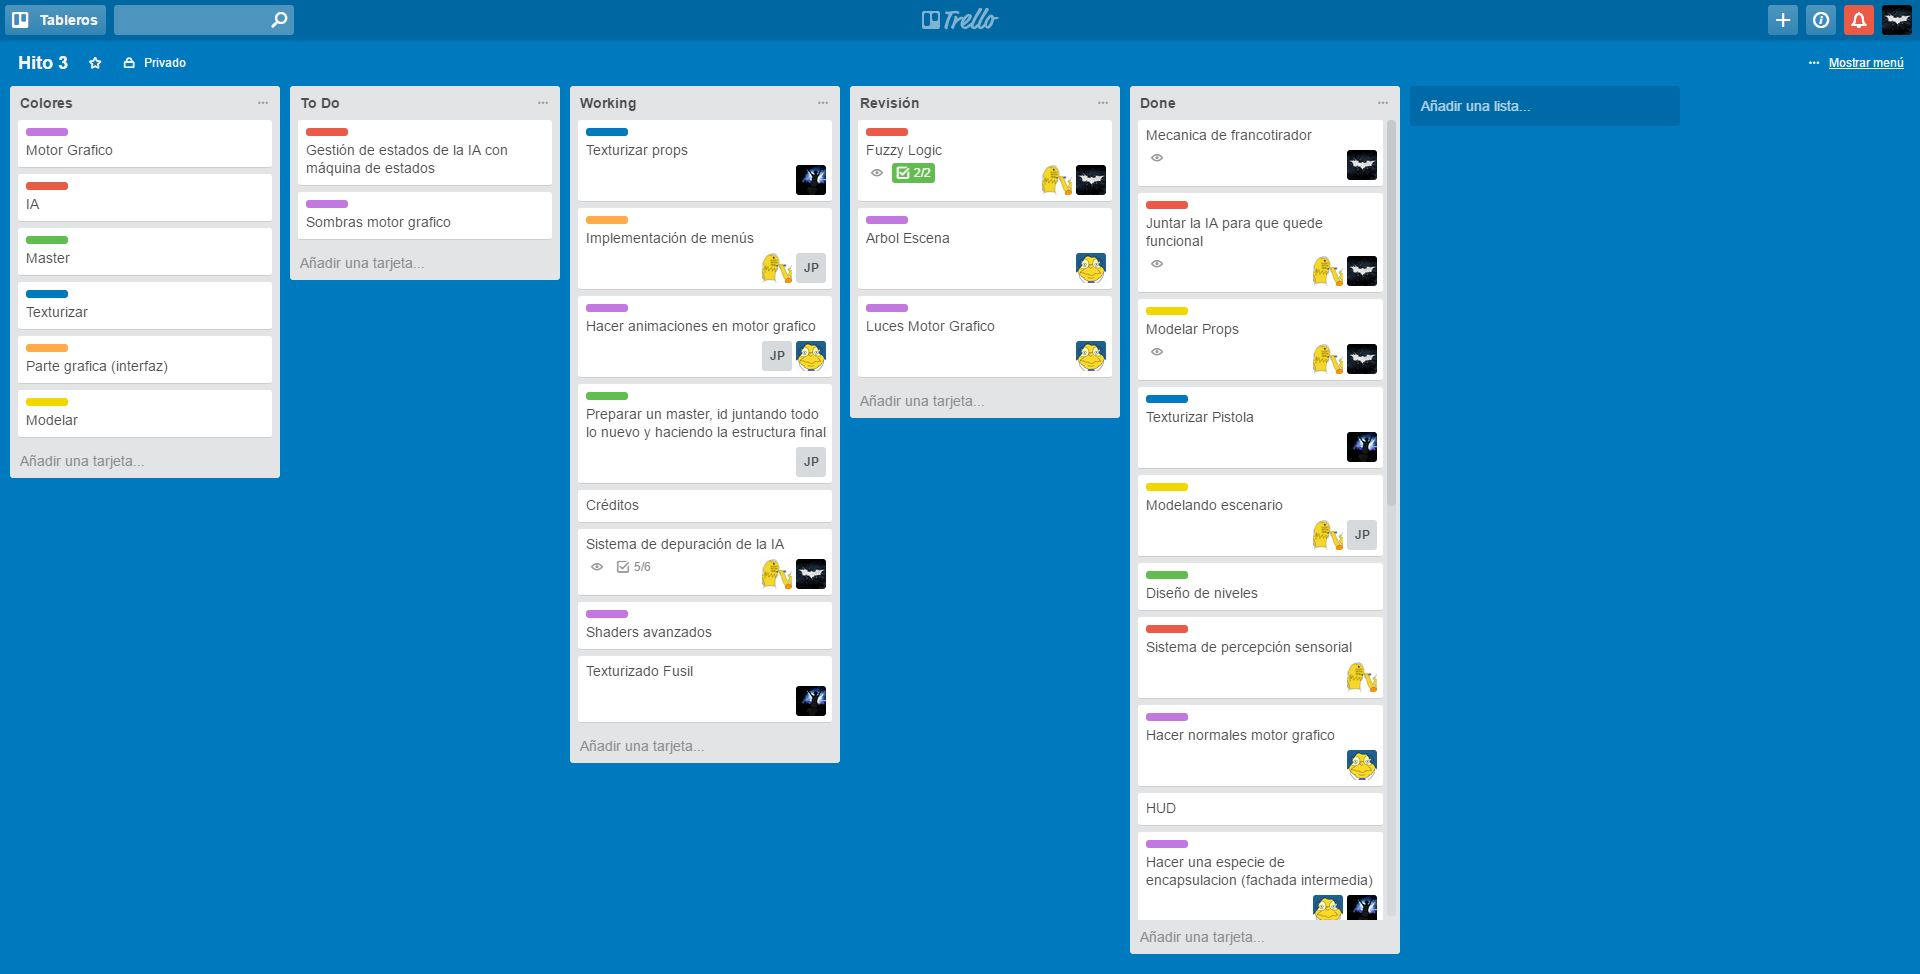
\includegraphics[scale=0.28]{imagenes/trello.jpg}
		\caption{Captura de pantalla de un tablero de \textit{Trello} de un proyecto anterior.}
		\label{trello}
	\end{center}
\end{figure}

El \ac{TFG} ha sido desarrollado usando la herramienta de gestión de proyectos \textit{Trello}, que nos permite crear tableros, etiquetas para las tareas y columnas en las que colocarlas. \textit{Trello} aporta una gran multitud de opciones con la que gestionar nuestros trabajos, como dividir las tareas en subtareas, clasificarlas por grupos o ponerles fechas límite o \textit{deadlines}.
\\

\textit{Trello} es una herramienta muy útil que he usado en anterioridad en otros trabajos y que resulta muy cómoda a la hora de gestionar el trabajo del proyecto.

\section{Control de versiones y repositorio}
	
Puesto que este es un trabajo individual no es necesario usar un sistema de control de versiones, no obstante, para mayor seguridad y para tener todo el contenido del proyecto disponible en Internet se ha decidido crear un repositorio en \textit{Github}.
De este modo siempre habrá una copia de seguridad disponible, además de que se puede volver a un momento anterior del proyecto si es necesario.
\\

El enlace del repositorio es el siguiente:
\\

\url{https://github.com/JoseLuisMunozP/TFG}

	
	
	
	
	
	
	
\begin{comment}


\begin{description}
\item[Índice de contenidos:] (obligatorio siempre) se incluirá un índice de las secciones de las que se componga el documento, la numeración de las 
divisiones y subdivisiones utilizarán cifras arábigas (según UNE 50132:1994) y harán mención a la página del documento donde se ubiquen.
\item[Índice de figuras:] si el documento incluye figuras se podrá incluir también un índice con su relación, indicando la página donde se ubiquen.
\item[Índice de tablas:] en caso de existir en el texto, ídem que el anterior.
\item[Índice de abreviaturas, siglas, símbolos, etc.:] en caso de ser necesarios se podrá incluir cada uno de ellos.
\end{description}
\item[Cuerpo del documento:] en el contenido del documento se da flexibilidad para su organización y se puede estructurar en las secciones que se considere. En todo caso obligatoriamente se deberá, al menos, incluir los siguientes contenidos:
\begin{description}
\item[Introducción:] donde se hará énfasis a la importancia de la temática, su vigencia y actualidad; se planteará el problema a investigar, así como el propósito o finalidad de la investigación.
\item[Marco teórico o Estado del arte:] se hará mención a los elementos conceptuales que sirven de base para la investigación, estudios previos relacionados con el problema planteado, etc.
\item[Objetivos:] se establecerá el objetivo general y los específicos.
\item[Metodología:] se indicará el tipo o tipos de investigación, las técnicas y los procedimientos que serán utilizados para llevarla a cabo; se identificará la población y el tamaño de la muestra así como las técnicas e instrumentos de recolección de datos.
\item[Resultados:] incluirá los resultados de la investigación o trabajo, así como el análisis y la discusión de los mismos.
\end{description}
\item[Conclusiones:] obligatoriamente se incluirá una sección de conclusiones donde se realizará un resumen de los objetivos conseguidos así como de los resultados obtenidos si proceden.
\item[Bibliografía y referencias:] se incluirá también la relación de obras y materiales consultados y empleados en la elaboración de la memoria del \ac{TFG}/\ac{TFM}. La bibliografía y las referencias serán indexadas en orden alfabético (sistema nombre y fecha) o se numerará correlativamente según aparezca (sistema numérico). Se empleará la familia 1 como tipo de letra. Podrá utilizarse cualquier sistema bibliográfico normalizado predominante en la rama de conocimiento, estableciéndose como prioritarios el sistema ISO 690, sistema \ac{APA}  o Harvard (no necesariamente en ese orden de preferencia). En esta plantilla Latex se propone usar el estilo \ac{APA} indicándolo en la línea correspondiente como 
\begin{verbatim}
\bibliographystyle{apalike}
\end{verbatim}


\item[Anexos:] se podrá incluir los anexos que se consideren oportunos.
\end{comment}




\chapter{Cuerpo del trabajo}

En este apartado desarrollaré en detalle todo el proceso de la creación del videojuego, se dividirá en las siguientes partes:

\begin{enumerate}
	\item Un apartado donde hablaré de las herramientas disponibles, así como la elección que se ha hecho entre todas ellas y su justificación.
	\item Una sección donde estará redactado el \ac{GDD}, en el que hablaré del juego y todas las características del mismo que van a ser implementadas.
	\item Por último, un apartado donde hablaré del desarrollo y la implementación del videojuego, acompañado de explicaciones e imágenes para que se puede apreciar que se ha hecho y de que manera.

\end{enumerate}

\section{Análisis y elección de herramientas para el desarrollo}

En el desarrollo de este proyecto se van a necesitar varios programas con distintas funcionalidades, quiero destacar entre ellos un programa que sea el \textbf{motor del videojuego}, otro que sea para \textbf{modelar} y por último uno que sirva para \textbf{texturizar}.

\subsection{Motor de videojuegos}

Los \textbf{motores de videojuegos} o \textbf{\textit{Game engines}} son \textit{software} diseñados para la creación y desarrollo de videojuegos, ya sea para juegos móvil, para consolas o para ordenadores. Estos motores suelen proveer todo lo necesario para la creación de videojuegos, como motores de físicas para el calculo colisiones o \textit{renderers} para la visualización de los gráficos 2D o 3D.
\\



Hay un número enorme de motores de videojuegos (como podemos apreciar en la imagen a continuación), por lo que para la elección se han tenido en cuenta sólo los dos motores de videojuego comerciales más utilizados en la industria, que son \textbf{\textit{Unity}} y \textbf{\textit{Unreal Engine 4}}.
	
	\begin{figure}[H]
		
				\vspace{-10pt}
		\begin{center}
			
			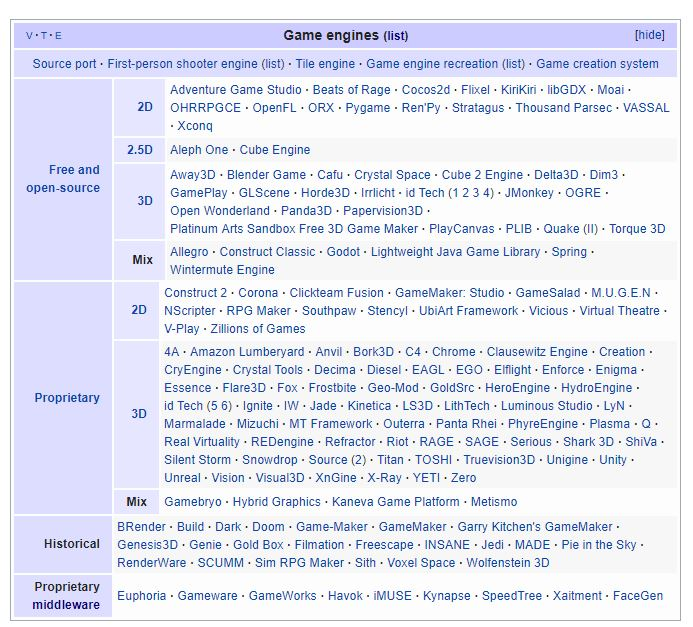
\includegraphics[width=0.85\textwidth]{imagenes/listaMotores.jpg}
			\caption{Lista de grandes motores de juego y sus licencias.}
		\end{center}
		\vspace{-40pt}
	\end{figure}
	
\subsubsection{\textit{Unity}}

\textbf{\textit{Unity}} es un motor de videojuegos creado por \textit{\textbf{Unity Technologies}} y disponible para Windows, macOS y Linux. Unity tiene dos versiones: \textit{Unity Professional} y \textit{Unity Personal}.
\\

\begin{wrapfigure}{i}{0.5\textwidth}
					\vspace{-10pt}
	\begin{center}
						\vspace{-10pt}
		\includegraphics[width=0.55\textwidth]{imagenes/unityLogo.png}
		\caption{Logo de \textit{Unity}.}
						\vspace{-10pt}
	\end{center}
					\vspace{-30pt}
\end{wrapfigure}


\textit{Unity} puede usarse con gran variedad de \textit{software}, como \textit{Blender},\textit{ 3ds Max}, \textit{Maya}, \textit{ZBrush}, \textit{Photoshop}, etc. Los cambios que se realicen a los objetos creados con estos programas se actualizan automáticamente en todo el proyecto sin necesidad de volver a importarlos.
\\


Hoy en día \textit{Unity} tiene un peso muy importante en la industria a la hora de desarrollar juegos, muchos grandes proyectos deciden usar este motor para sus videojuegos, como \textit{\textbf{Hearthstone}} o \textit{\textbf{Furi}}, juegos de gran éxito de ventas y crítica.
\\

No obstante, \textit{Unity} tiene más peso en el sector móvil que en el desarrollo de juegos para ordenadores personales, así que ese motivo junto con la falta de experiencia previa con el motor ha hecho que me decante por \textit{Unreal Engine 4} a la hora de desarrollar el \ac{TFG}.




\subsubsection{\textit{Unreal Engine 4}}
	
\textbf{\textit{Unreal Engine}} es un motor de videojuegos creado por la compañía \textbf{\textit{Epic Games}}, desarrolladora de juegos como \textbf{\textit{Gears of war}} o \textbf{\textit{Unreal Tournament}}.
\\


\begin{wrapfigure}{i}{0.6\textwidth}
	\vspace{-30pt}
	\begin{center}
		\vspace{-10pt}
		
\includegraphics[width=0.55\textwidth]{imagenes/unrealLogo.jpg}
		\caption{Logo de \textit{Unreal Engine 4}.}
	\vspace{-10pt}
	\end{center}
	\vspace{-30pt}
\end{wrapfigure}

La versión actual de \textit{Unreal} está programada en C++ y es compatible con OpenGL y con DirectX 11 y 12. Esta disponible para Windows, Linux y macOS. Además, \textit{Unreal Engine} ofrece herramientas para diseñadores y artistas facilitando la visualización de entornos o de construcciones, lo que ha permitido que \textit{Unreal} se use también en empresas de arquitectura o incluso animación.
\\

\textit{Unreal Engine} es muy utilizado en la industria, hasta el punto que grandes éxitos como los \textit{\textbf{Bioshock}}, \textit{\textbf{Outlast}} e incluso el reciente \textit{\textbf{PlayerUnknown's Battlegrounds}} usen este motor.
\\

\textbf{He decidido usar este motor} precisamente por el gran uso que se tiene de él por parte de las empresas, además de que ya tenía experiencia previa con él, lo que me permitirá acabar con un producto final más redondo. También ha sido determinante en mi elección el sobresaliente acabado final que otorga \textit{Unreal} a los juegos, muy por encima de la mayoría de motores de videojuegos.
\\

\subsection{Programa de modelado}

En gráficos 3D por ordenador, el \textbf{modelado 3D} es el proceso de desarrollo de una una representación matemática de cualquier objeto tridimensional a través de un \textbf{\textit{software} especializado}. Estos modelos pueden ser usado en muchas áreas, como el cine o en la impresión 3D, sin embargo, la utilidad que estamos buscando nosotros es de desarrollo modelos para \textbf{videojuegos}.
\\

\begin{figure}[H]
	
	\vspace{-10pt}
	\begin{center}
		
		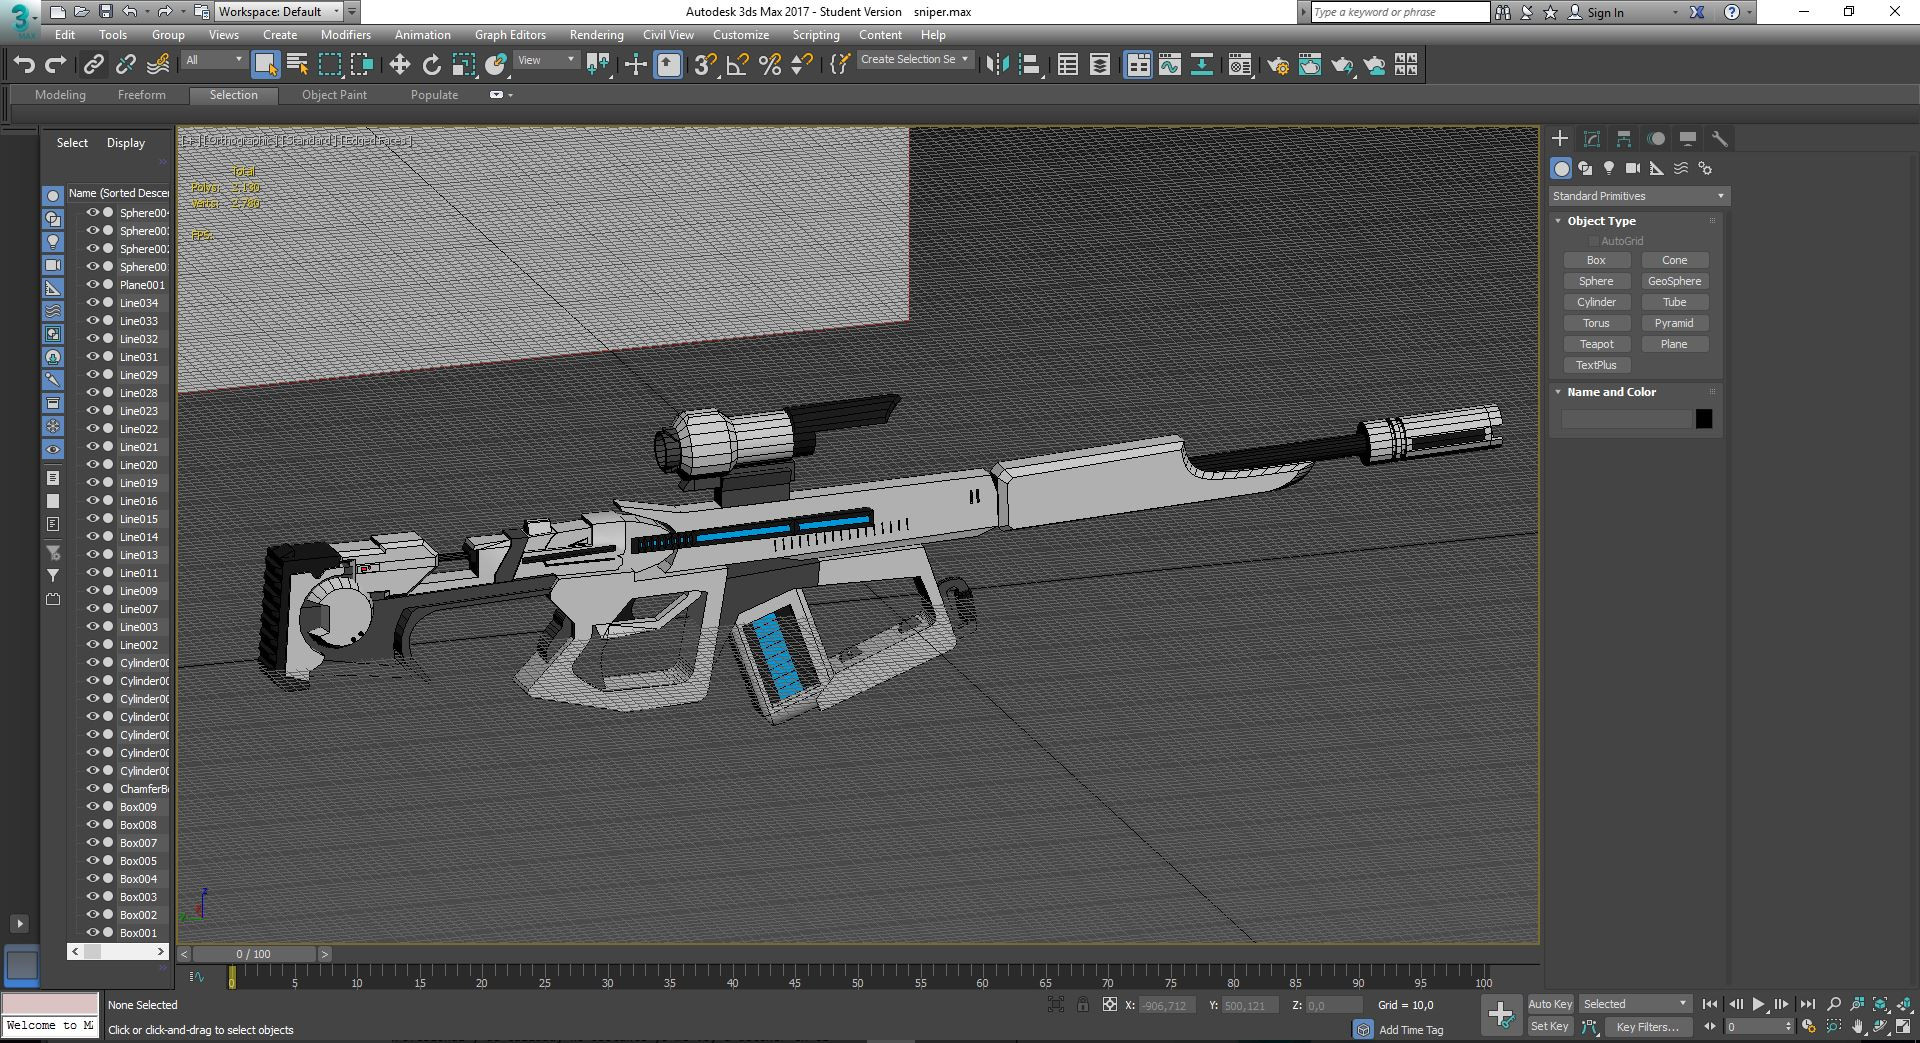
\includegraphics[width=0.9\textwidth]{imagenes/ejemploModelo.jpg}
		\caption{Imagen de un modelo desarrollado por \textit{3ds Max}.}
	\end{center}
	\vspace{-40pt}
\end{figure}

Hay muchos programas de modelado que permiten realizar recursos con un acabado profesional y de calidad, no obstante yo me voy a detener en el \textbf{\textit{Blender}}, el \textbf{\textit{3ds Max}} y el \textbf{Maya\textit{}}, ya que son tres \textit{software} de modelado muy utilizados en la industria.
\\

\subsubsection{\textit{Blender}}

\textit{\textbf{Blender}} es un programa multiplataforma, dedicado especialmente al modelado, iluminación, renderizado, animación y creación de \textbf{gráficos tridimensionales}. \textit{Blender} es un programa de \textbf{software libre}, compatible con \textit{Windows}, \textit{macOS}, \textit{GNU/Linux}, \textit{Solaris}, \textit{FreeBSD} e \textit{IRIX}.
\\

\begin{wrapfigure}{i}{0.6\textwidth}
	\vspace{-30pt}
	\begin{center}
		\vspace{-10pt}
		
\includegraphics[width=0.55\textwidth]{imagenes/blenderLogo.png}
		\caption{Logo de \textit{Blender}.}
		\vspace{-10pt}
	\end{center}
	\vspace{-30pt}
\end{wrapfigure}

\textit{Blender} es un programa muy usado en la industria por pequeñas empresas, ya que el hecho de que sea gratuito lo hace muy apetecible para proyectos de poco presupuesto. También es usado en la industria del cine en películas como \textbf{Spider-man 2} o \textbf{Capitán América: El Soldado de Invierno}.
\\

No obstante, en mi opinión y experiencia previa es un programa mucho más limitado e incómodo que otros \textit{software} de modelado como Maya o 3ds Max, y como puedo utilizar estos dos programas gracias a mi licencia de estudiante no usaré Blender para la realización de este proyecto.
\\

\subsubsection{\textit{Autodesk Maya}}
	
\textbf{\textit{Autodesk Maya}} es un programa dedicado al desarrollo de gráficos 3D por ordenador, efectos especiales y animación creado por \textit{Autodesk}. Esta disponible para \textit{Windows}, \textit{GNU/Linux} y \textit{macOS}.
\\

\begin{wrapfigure}{l}{0.6\textwidth}
	\vspace{-30pt}
	\begin{center}
		\vspace{-30pt}
		
\includegraphics[width=0.35\textwidth]{imagenes/mayaLogo.jpg}
		\caption{Logo de \textit{Autodesk Maya}.}
		\vspace{-20pt}
	\end{center}
	\vspace{-30pt}
\end{wrapfigure}

Este \textit{software} ha tenido un impacto impresionante en la industria del cine, siendo usado en grandes producciones como \textit{\textbf{Jurassic Park}} o \textbf{\textit{Terminator 2}}. Hoy en día prácticamente todas las grandes producciones de Hollywood usan \textit{Maya} para sus efectos especiales.
\\

Sin embargo, aunque este programa tiene una importancia vital en el mundo del cine, \textit{3ds Max} es mucho más usado en el mundo del desarrollo de videojuegos, además, mi experiencia con Maya es mucho más reducida que con 3ds Max.
\\	
	
\subsubsection{\textit{Autodesk 3ds Max}}
	
	
	\begin{wrapfigure}{r}{0.6\textwidth}
		\vspace{-30pt}
		\begin{center}
			\vspace{-30pt}
			
\includegraphics[width=0.35\textwidth]{imagenes/3dsMaxLogo.jpg}
			\caption{Logo de \textit{Autodesk 3ds Max}.}
			\vspace{-20pt}
		\end{center}
		\vspace{-30pt}
	\end{wrapfigure}

\textbf{\textit{Autodesk 3ds Max}} es un programa de creación de gráficos y animación 3D también desarrollado por \textit{Autodesk}. Es uno de los programas de modelado y animación 3D usados en la creación de videojuegos.
\\
	
Aunque es un programa principalmente usado en la industria del videojuego, también ha sido muy usado para anuncios, programas de televisión o películas, destacando \textbf{\textit{Avatar}} o \textbf{\textit{Spider-man 3}}.
\\

\textbf{Esta es la opción que he elegido}, ya que, como he dicho anteriormente, es el \textit{software} más utilizado a día de hoy en el desarrollo de videojuegos. Además, también es el programa con el que tengo más experiencia modelando, por lo que puedo conseguir modelos de calidad en menos tiempo del que necesitaría usando otros programas.
\\
	
	
	
	
	\subsection{Programa de texturizado}
	
\textbf{Texturizar} consiste en crear una \textbf{imagen de mapa de bits} para que cubra la superficie de un objeto virtual, es decir, un modelo. De este modo se le añade detalle al modelo, haciendo que se asemeje más a un objeto real.
\\

	\begin{figure}[H]
		
		\vspace{-10pt}
		\begin{center}
			
			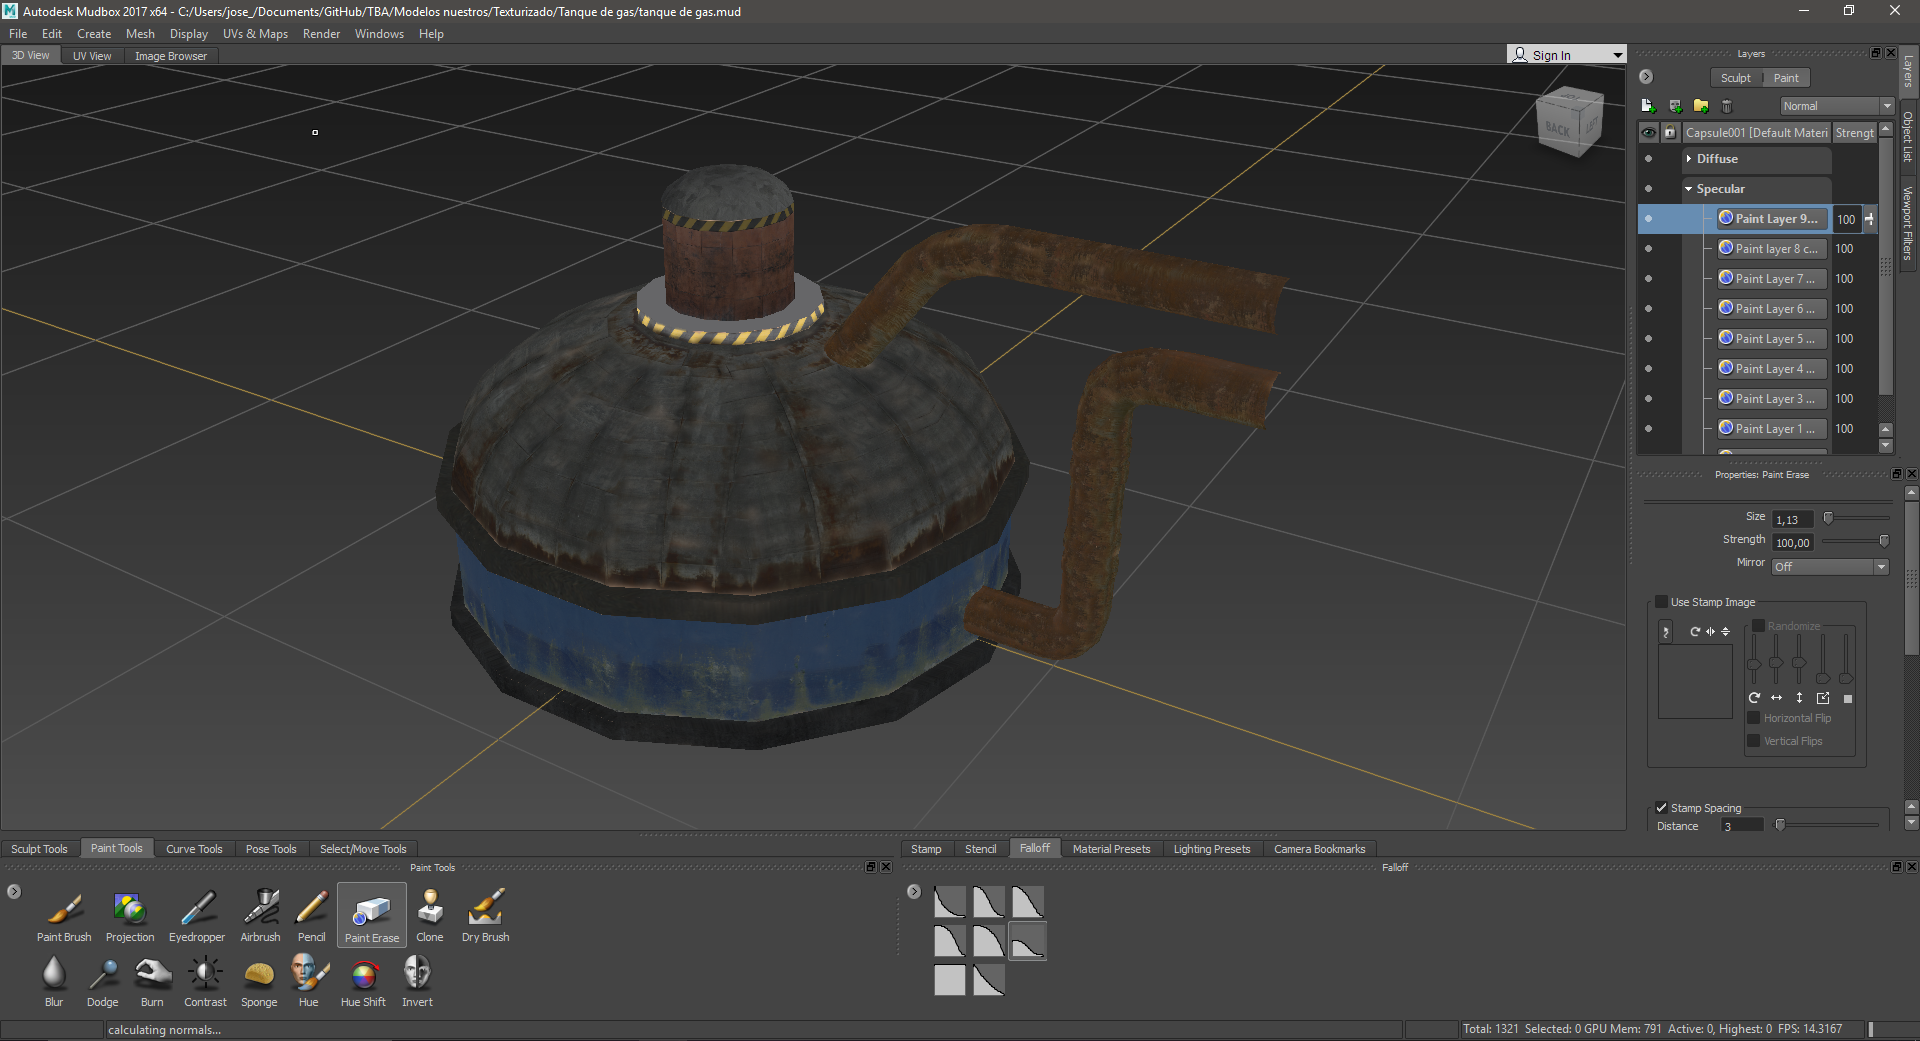
\includegraphics[width=0.9\textwidth]{imagenes/MudboxCapture.png}
			\caption{Imagen de un modelo siendo texturizado en \textit{Mudbox}.}
		\end{center}
		\vspace{-40pt}
	\end{figure}
	
Hay diversos programas que permiten texturizar, incluso algunos que he mencionado anteriormente como 3ds Max tienen herramientas para el texturizado, no obstante existen \textit{software} más especializados y que ofrecen un abanico de posibilidades mayor, como son \textbf{Substance painter} o \textbf{Mudbox}.
\\
	
	\subsubsection{\textit{Substance painter}}
	
	\textit{\textbf{Substance painter}} es un programa de texturizado que está creciendo cada vez más dentro del mercado, que consigue resultados impresionantes de manera sencilla e intuitiva. Está disponible en \textit{Windows}, \textit{macOS} y \textit{Linux}.
	\\
	
	\begin{wrapfigure}{i}{0.6\textwidth}
		\vspace{-30pt}
		\begin{center}
			\vspace{-10pt}
			
\includegraphics[width=0.5\textwidth]{imagenes/substanceLogo.png}
			\caption{Logo de \textit{Substance painter}.}
			\vspace{-10pt}
		\end{center}
		\vspace{-30pt}
	\end{wrapfigure}
	
Una pega del \textit{Substance painter} es que, aunque está creciendo a buen ritmo, su uso en la industria sigue siendo menor. También, al ser un programa no muy utilizado, se pueden encontrar menos recursos y tutoriales para el aprendizaje que los que encuentras para otros programas.
\\
	
Debido a estas razones y a la falta total de experiencia, \textit{Substance painter} ha sido descartado para el uso del producto final, sin embargo, me ha parecido lo suficientemente interesante y destacable como para mencionarlo en esta memoria.
\\


	\subsubsection{\textit{Autodesk Mudbox}}

\textit{\textbf{Autodesk Mudbox}} es un programa de modelado 3D, texturizado y pintura digital desarrollado por \textit{Autodesk}, fue usado por primera vez en la película \textbf{\textit{King Kong} (2005)}. Mudbox funciona perfectamente en sistemas operativos como \textit{Windows}, \textit{Linux} y \textit{macOS}.
\\

\begin{wrapfigure}{r}{0.6\textwidth}
	\vspace{-30pt}
	\begin{center}
		\vspace{-10pt}
		
\includegraphics[width=0.4\textwidth]{imagenes/mudboxLogo.png}
		\caption{Logo de \textit{Autodesk Mudbox}.}
		\vspace{-10pt}
	\end{center}
	\vspace{-30pt}
\end{wrapfigure}

Al ser un programa de \textit{Autodesk}, \textit{Mudbox} tiene mucho más uso en la industria que el que tiene \textit{Substance painter}, siendo mucho más atractivo aprender a usarlo a la hora de incorporarse al mundo laboral el día de mañana.
\\

He decidido \textbf{usar este \textit{software}} precisamente por eso, ya que puede aportarme mucho más en el futuro que \textit{substance painter}, por no hablar que ya tengo cierta base a la hora de usarlo aprendida a lo largo del último año de carrera.
\\


\section{\textit{Game Desing Document} (GDD)}
	
El\textbf{ Documento de Diseño del Juego} (o \textit{Game Design Document}) es el documento en el que se sintetiza todos los componentes y características del juego (concepto, historia, género, niveles...)

Hay muchas maneras y plantillas a la hora de realizar un GDD, no hay una manera fija de esquematizar las diferentes partes del mismo, así que yo voy a seguir el siguiente orden:

\begin{enumerate}
	\item Título y concepto del juego.
		\subitem Título.
		\subitem Historia y argumento.
		\subitem Conjunto de características.
	\item Desarrolladores y género.
		\subitem Desarrolladores.
		\subitem Género.
	\item Plataforma.
	\item Jugabilidad y contenido.
		\subitem Jugabilidad.
		\subitem Objetivos del juego.
		\subitem Progresión.
		\subitem Acciones del personaje.
		\subitem Mecánicas.
		\subitem Controles.
		\subitem Nivel del juego.
		\subitem Apariencia del juego.
	\item Tecnología.
	\item Público.
\end{enumerate}

\subsection{Título y concepto del juego}

\subsubsection{Título}

Lorem Ipsum es simplemente el texto de relleno de las imprentas y archivos de texto. Lorem Ipsum ha sido el texto de relleno estándar de las industrias desde el año 1500, cuando un impresor (N. del T. persona que se dedica a la imprenta) desconocido usó una galería de textos y los mezcló de tal manera que logró hacer un libro de textos especimen. No sólo sobrevivió 500 años, sino que tambien ingresó como texto de relleno en documentos electrónicos, quedando esencialmente igual al original. Fue popularizado en los 60s con la creación de las hojas "Letraset", las cuales contenian pasajes de Lorem Ipsum, y más recientemente con software de autoedición, como por ejemplo Aldus PageMaker, el cual incluye versiones de Lorem Ipsum.
\\

\subsubsection{Historia y argumento}

Nos despertamos desorientados en una pequeña celda oscura y mugrienta, no sabemos que hacemos ahí, solo que\textbf{ estamos en peligro}.
\\

Según escapes de la celda y avances en el juego verás que estas atrapado en una casa de la cual no puedes salir, dónde pasan cosas extrañas, \textbf{tienes que escapar cuanto antes de ahí}.

\subsubsection{Conjunto de características}

Las principales características del juego son:

\begin{itemize}
	\item Ambientación oscura y realista.
	\item Compatible con \textbf{Oculus Rift}.
	\item Desarrollado con \textbf{Unreal Engine 4}
	\item Diseño de niveles centrado en descubrir nuevas localizaciones y salas.
	\item Nivel lleno de detalles.
	\item Mecánicas sencillas y fáciles de aprender.
	\item Diseño sonoro destacable e inmersivo.
\end{itemize}


\subsection{Desarrolladores y género}

\subsubsection{Desarrolladores}

\textbf{\nombreJuego} es un videojuego desarrollado individualmente por José Luis Muñoz Periñán como Trabajo de Fin de Grado de la carrera ingeniería multimedia. Tiene fines puramente académicos y no está previsto ningún uso comercial del producto final.

\subsubsection{Género}

\nombreJuego pertenece al género de los juegos de miedo o \textbf{\textit{survival horror}}.
\\

El juego es una aventura en primera persona inspirada en muchos juegos de miedo de gran éxito en los últimos años, como \textit{Outlast}, \textit{P.T.} o el más reciente \textit{Resident Evil VII}. Se mirarán también como funcionan algunos videojuegos de miedo desarrollados o adaptados para realidad virtual, ya que \nombreJuego estará totalmente adaptado para realidad virtual.
\\

La atmósfera, diseño de mecánicas, apartado artístico y demás características del videojuego estarán enfocadas de acuerdo al género del juego.
\\

\subsection{Plataforma}

\nombreJuego es un videojuego creado en \textit{Unreal Engine 4} desarrollado para ordenadores personales y compatible con las gafas\textit{Oculus Rift}. Cabe destacar que el juego será perfectamente jugable dispongas o no del dispositivo de realidad virtual.
\\

\subsection{Jugabilidad y contenido}

\subsubsection{Jugabilidad}

La jugabilidad será la semejante a la que estamos acostumbrados en los juegos de terror moderno. El protagonista será alguien indefenso y sin recursos ante una situación tenebrosa y que le supera. Unicamente podrá investigar los alrededores e interactuar con el entorno para intentar salir de esa situación. 
\\

Será un juego con mecánicas limitadas para aumentar la sensación de indefensión del jugador e incrementar el terror que el juego provoca.
\\

\subsubsection{Objetivos del juego}

Como he dicho anteriormente, el protagonista está encerrado en una celda de una casa tenebrosa y su objetivo es intentar salir de ahí por todos los medios posibles. A lo largo del juego habrá varios obstáculos que intentarán impedir que alcance su objetivo, como puzzles o momentos de tensión que tendrá que superar usando su ingenio y los objetos que encuentre en el escenario.
\\

\subsubsection{Progresión}

Lorem Ipsum es simplemente el texto de relleno de las imprentas y archivos de texto. Lorem Ipsum ha sido el texto de relleno estándar de las industrias desde el año 1500, cuando un impresor (N. del T. persona que se dedica a la imprenta) desconocido usó una galería de textos y los mezcló de tal manera que logró hacer un libro de textos espécimen. No sólo sobrevivió 500 años, sino que también ingresó como texto de relleno en documentos electrónicos, quedando esencialmente igual al original.
\\

\subsubsection{Acciones del personaje}

El jugador podrá moverse libremente por todo el escenario sin límites, esto es importante ya que el entorno juega un papel importantísimo en el juego, ya que el jugador también podrá coger y usar los objetos de interés que encuentre en el nivel. Por último el jugador también podrá inspeccionar detalladamente algunos objetos específicos que tengan pistas más escondidas moviéndolos y girándolos enfrente suya.
\\

\subsubsection{Mecánicas}

\subsubsection{Controles}

\subsubsection{Nivel del juego}

\subsubsection{Flujo del juego}

\subsubsection{Apariencia del juego}

\subsection{Tecnología}

\subsection{Público}

%input{capitulos/resultados}
%input{capitulos/conclusiones}

\chapter{Bibliografía}
\label{bibliografia}

Videojuego según la Wikipedia:

\url{https://es.wikipedia.org/wiki/Videojuego}

El género de terror o \textit{survival horror}:

\url{https://es.wikipedia.org/wiki/Survival_horror}

Outlast:

\url{https://es.wikipedia.org/wiki/Outlast}

P.T.:

\url{https://en.wikipedia.org/wiki/P.T._(video_game)}

Alien: Isolation:

\url{https://es.wikipedia.org/wiki/Alien:_Isolation}

Motor de videojuegos:

\url{https://en.wikipedia.org/wiki/Game_engine}

Unity:

\url{https://es.wikipedia.org/wiki/Unity_(motor_de_juego)}

Unreal Engine 4:

\url{https://es.wikipedia.org/wiki/Unreal_Engine}

\url{https://www.unrealengine.com/en-US/blog}

Modelado 3D:

\url{https://es.wikipedia.org/wiki/Modelado_3D}

Blender:

\url{https://es.wikipedia.org/wiki/Blender}

Maya:

\url{https://es.wikipedia.org/wiki/Autodesk_Maya}

3ds Max:

\url{https://es.wikipedia.org/wiki/Autodesk_3ds_Max}

\url{https://en.wikipedia.org/wiki/Autodesk_3ds_Max}

Texturizado:

\url{https://en.wikipedia.org/wiki/Texture_mapping}

\url{https://es.wikipedia.org/wiki/Textura_(gr%C3%A1ficos_por_computadora)}
	
Substance painter:

\url{https://www.allegorithmic.com/products/substance-painter}

Mudbox:

\url{https://en.wikipedia.org/wiki/Autodesk_Mudbox}

GDD:

\url{http://www.hagamosvideojuegos.com/2015/06/como-crear-un-documento-de-diseno-de.html}

\url{https://eldocumentalistaudiovisual.com/2015/02/06/documentacion-en-videojuegos-documento-de-diseno-gdd/}


\chapter*{Lista de Acrónimos}
% fichero para poner los acrónimos
%para escribir un acrónimo nuevo, seguir el siguiente protocolo: (POR EJEMPLO PARA PONER EL ACRÓNIMO IEEE)
%- En el texto, poned \ac{IEEE}
%- En el fichero acrónimos.tex, poner la siguiente enTrada:
% \acrodef{IEEE}{Institute of Electrical and Electronics Engineers}
% IEEE: Institute of Electrical and Electronics Engineers

%Además de \ac{IEEE} se pueden usar otras fórmulas en el texto para variar el comportamiento del paquete de acrónimos:
% Por ejemplo:
% acf{} hace que siempre aparezca el texto completo del acrónimo correspondiente. (fórmula larga y corta)
% acl{} hace que Solo aparezca la fórmula larga
% acs{} hace que aparezca obligatoriamente la fórmula corta
% acp{} incluye el plural del acrónimo.
% acs{} hace que aparezca la versión córta del acrónimo.
% acresetall{} resetea todos los acrónimos de forma que se establecen como “no usados”.
% acused{} marca el acrónimo como “usado”.


\acrodef{IEEE}{Institute of Electrical and Electronics Engineers}
IEEE: Institute of Electrical and Electronics Engineers

\acrodef{GDD}{Documento de diseño del juego}
GDD: Documento de diseño del juego

\acrodef{MIT}{Instituto Tecnológico de Massachusetts}
MIT: Instituto Tecnológico de Massachusetts

\acrodef{TFG}{Trabajo Final de Grado}
\acrodefplural{TFG}[TFG]{Trabajos Finales de Grado} %NOTA: chequea cómo se hace para usar un plural en un acrónimo, en su versión larga. En su versión corta, Los acrónimos, en castellano, NUNCA se escriben con una "s" al final. ver http://www.rae.es/consultas/plural-de-las-siglas-las-ong-unos-dvd
TFG: Trabajo Final de Grado


\acrodef{TFM}{Trabajo Final de Master}
TFM: Trabajo Final de Master

\acrodef{EPS}{Escuela Politécnica Superior} %NOTA: este acrónimo NO aparecerá en el capítulo de la lista de acrónimos al carecer de su entradilla. Esto se hace en algunos casos, cuando ponerlo en la lista de acrónimos no es aclaratorio.

\acrodef{APA}{American Psychological Association} %NOTA: este acrónimo NO aparecerá en el capítulo de la lista de acrónimos al carecer de su entradilla.



\addcontentsline{toc}{chapter}{Lista de Acrónimos}


\begin{comment}
%\nocite{*} %incluye TODOS los documentos de la base de datos bibliográfica sean o no citados en el texto
\bibliography{bibliografia/bibliografia}\addcontentsline{toc}{chapter}{Bibliografía} %sustituir bibliografía con el nombre del fichero bibtex con la bibliografía
\bibliographystyle{apalike}
%
\appendix
\chapter{Anexo I}
Aquí vendría en anexo I 
\end{comment}

\end{document}
